\documentclass[12pt,a4paper]{report}

% ==============================================================================
% 1. PACKAGES ET ENCODAGE CONFORMES AU GUIDE EMSI (ANNEXE B)
% ==============================================================================
\usepackage[utf8]{inputenc}
\usepackage[T1]{fontenc}
\usepackage[french]{babel}
\usepackage{mathptmx} % Police Times New Roman 12pt conforme au guide (Annexe B)
\usepackage[top=2.5cm, bottom=2.5cm, left=2.5cm, right=2.5cm]{geometry} % Marges 2.5 cm (Annexe B)
\usepackage{setspace}
\onehalfspacing % Interligne 1.5 ligne (Annexe B)
\usepackage{parskip}
\setlength{\parindent}{0.8cm} % Alinéa de 1ère ligne : 0.8 cm (Annexe B)
\setlength{\parskip}{6pt}      % Espacement avant et après les paragraphes : 6pt (Annexe B)

% Packages graphiques, couleurs et tableaux
\usepackage{graphicx}
\usepackage{pdflscape}
\usepackage{float}
\usepackage[section]{placeins}
\graphicspath{{images/}{./}}
\usepackage{xcolor}
\usepackage{booktabs}
\usepackage{tabularx}
\usepackage{array}
\usepackage{multirow}
\usepackage{colortbl}
\usepackage{tikz}
\usetikzlibrary{calc,positioning,shapes.geometric}
\usepackage{tcolorbox}
\tcbuselibrary{skins,breakable}

% Packages d'en-tête et pied de page
\usepackage{fancyhdr}
\usepackage{titlesec}
\usepackage{caption}
\usepackage{chngcntr}
\counterwithout{figure}{chapter}
\counterwithout{table}{chapter}

% Configuration des légendes selon l'Annexe B :
% Tableaux : titre au-dessus | Figures : titre en-dessous
\captionsetup[table]{position=top, skip=6pt, labelfont=bf, textfont=it}
\captionsetup[figure]{position=bottom, skip=6pt, labelfont=bf, textfont=it}

% Package listings pour les extraits de code source
\usepackage{listings}
\definecolor{codebg}{rgb}{0.97,0.97,0.98}
\definecolor{codeblue}{rgb}{0.13,0.38,0.72}
\definecolor{codegreen}{rgb}{0.12,0.55,0.24}
\definecolor{codegray}{rgb}{0.45,0.45,0.45}
\lstset{
  backgroundcolor=\color{codebg},
  basicstyle=\ttfamily\footnotesize,
  breaklines=true,
  captionpos=b,
  commentstyle=\color{codegreen},
  keywordstyle=\color{codeblue}\bfseries,
  stringstyle=\color{red!70!black},
  numbers=left,
  numberstyle=\tiny\color{codegray},
  numbersep=8pt,
  frame=single,
  rulecolor=\color{gray!30},
  tabsize=2,
  showstringspaces=false,
  extendedchars=true,
  inputencoding=utf8,
  literate=%
    {é}{{\'e}}1
    {è}{{\`e}}1
    {ê}{{\^e}}1
    {ë}{{\"e}}1
    {à}{{\`a}}1
    {â}{{\^a}}1
    {ù}{{\`u}}1
    {û}{{\^u}}1
    {ç}{{\c{c}}}1
}

% Liens hypertexte
\usepackage[colorlinks=true, linkcolor=black, citecolor=blue!80!black, urlcolor=blue!70!black]{hyperref}

% Couleurs institutionnelles EMSI
\definecolor{EmsiRed}{RGB}{185, 20, 26}
\definecolor{EmsiGreen}{RGB}{20, 120, 70}
\definecolor{LightGray}{RGB}{245, 245, 248}

% ==============================================================================
% 2. CONFIGURATION DE LA NUMÉROTATION CONFORME AU TEMPLATE EMSI (PAGES 4, 10, 13, 16, 20)
% ==============================================================================
% Numérotation décimale des sections : 1. Introduction, 2. Présentation, 3.1. Description...
\renewcommand{\thesection}{\arabic{section}}
\renewcommand{\thesubsection}{\arabic{section}.\arabic{subsection}}
\renewcommand{\thesubsubsection}{\arabic{section}.\arabic{subsection}.\arabic{subsubsection}}

% Formatage des titres (Annexe B : ni deux-points à la fin, ni soulignés, ni italiques)
\titleformat{\section}
  {\normalfont\bfseries\Large\color{black}}
  {\thesection.}{8pt}{}
\titlespacing*{\section}{0pt}{12pt}{6pt}

\titleformat{\subsection}
  {\normalfont\bfseries\large\color{black}}
  {\thesubsection.}{8pt}{}
\titlespacing*{\subsection}{0pt}{10pt}{4pt}

\titleformat{\subsubsection}
  {\normalfont\bfseries\normalsize\color{black}}
  {\thesubsubsection.}{8pt}{}
\titlespacing*{\subsubsection}{0pt}{8pt}{3pt}

% Style d'en-tête et pied de page (Annexe B : en-tête = titre du chapitre, pied de page = titre du projet + page)
\setlength{\headheight}{14.5pt}
\pagestyle{fancy}
\fancyhf{}
\renewcommand{\headrulewidth}{0.5pt}
\renewcommand{\footrulewidth}{0.5pt}
\fancyhead[L]{\small\nouppercase{\leftmark}}
\fancyfoot[L]{\small\itshape TutorAI -- Tuteur Adaptatif pour Élèves en Difficulté (6-15 ans)}
\fancyfoot[R]{\small\thepage}

\fancypagestyle{plain}{
  \fancyhf{}
  \renewcommand{\headrulewidth}{0pt}
  \renewcommand{\footrulewidth}{0.5pt}
  \fancyfoot[L]{\small\itshape TutorAI -- Tuteur Adaptatif pour Élèves en Difficulté (6-15 ans)}
  \fancyfoot[R]{\small\thepage}
}

% ==============================================================================
% 3. MACRO POUR LA PAGE DE GARDE DE CHAPITRE (CONFORME AUX PAGES 9, 12, 15, 19 DU TEMPLATE)
% ==============================================================================
\newcommand{\chaptercoverpage}[4][]{%
  \clearpage
  \thispagestyle{empty}%
  \refstepcounter{chapter}%
  \setcounter{section}{0}%
  \ifx&#1&%
    \addcontentsline{toc}{chapter}{Chapitre \thechapter\ : #2}%
    \markboth{Chapitre \thechapter\ : #2}{Chapitre \thechapter\ : #2}%
  \else
    \addcontentsline{toc}{chapter}{Chapitre \thechapter\ : #1}%
    \markboth{Chapitre \thechapter\ : #1}{Chapitre \thechapter\ : #1}%
  \fi
  
  \vspace*{2.0cm}
  \noindent
  \begin{center}
  \begin{tikzpicture}
    % Rectangle rouge EMSI conforme aux proportions de la maquette officielle
    \fill[EmsiRed] (0, 0) rectangle (7.6, 12.0);
    
    % Lettre 'C' majuscule géante
    \node[white, font=\fontsize{110}{110}\selectfont\rmfamily\bfseries, anchor=base west] at (0.2, 6.9) {C};
    
    % 'hapitre' aligné sur la même ligne de base que le C
    \node[white, font=\fontsize{24}{28}\selectfont\rmfamily\bfseries, anchor=base west] at (3.8, 6.9) {hapitre};
    
    % Numéro du chapitre géant centré en bas
    \node[white, font=\fontsize{125}{125}\selectfont\rmfamily\bfseries, anchor=base] at (3.8, 1.2) {#3};
    
    % Titre du chapitre positionné immédiatement à droite du bloc rouge
    \node[anchor=west, align=left, text width=7.4cm, font=\fontsize{26}{33}\selectfont\rmfamily\bfseries\color{black}] at (8.3, 6.9) {#2};
  \end{tikzpicture}
  \end{center}

  \vfill
  \clearpage
}

% ==============================================================================
% 4. INSERTION DES FIGURES ET PHOTOS DANS LE RAPPORT
% ==============================================================================
% Dans le corps du document, chaque figure est insérée via l'environnement standard :
% \begin{figure}[H]
%   \centering
%   \IfFileExists{votre_photo.png}{\includegraphics[width=0.85\textwidth]{votre_photo.png}}{...cadre de réservation...}
%   \caption{Titre de la figure}
%   \label{fig:...}
% \end{figure}
% Pour insérer votre photo, il vous suffit de déposer votre fichier (ex: photo.png ou photo.jpg)
% dans le dossier du rapport et d'indiquer son nom dans \includegraphics{...}.

% ==============================================================================
% DÉBUT DU DOCUMENT
% ==============================================================================
\begin{document}

% ------------------------------------------------------------------------------
% PAGE DE GARDE (REPRODUCTION STRICTEMENT CONFORME À LA CAPTURE DU MODÈLE - PAGE 1)
% ------------------------------------------------------------------------------
\begin{titlepage}
\thispagestyle{empty}

\begin{tikzpicture}[remember picture, overlay]
  % Polygone décoratif supérieur gauche (Rouge bordeaux EMSI)
  \fill[EmsiRed] (current page.north west) -- ++(11.5cm, 0) -- ++(-11.5cm, -9.0cm) -- cycle;
  \draw[white, line width=1.5pt] (current page.north west) ++(11.5cm, 0) -- ++(-11.5cm, -9.0cm);
  
  % Triangle inférieur droit (Rouge bordeaux EMSI)
  \fill[EmsiRed] (current page.south east) -- ++(-7.5cm, 0) -- ++(7.5cm, 6.0cm) -- cycle;
  \draw[white, line width=1.5pt] (current page.south east) ++(-7.5cm, 0) -- ++(7.5cm, 6.0cm);
\end{tikzpicture}

\vspace*{-0.6cm}
\begin{flushright}
  % LOGO EMSI OFFICIEL COMPLET (GRAPHISME + TEXTE INSTITUTIONNEL)
  \IfFileExists{logo_emsi.png}{%
    
\includegraphics[height=2.2cm,keepaspectratio]{logo_emsi.png}%
  }{%
    \IfFileExists{images/logo_emsi.png}{%
      
\includegraphics[height=2.2cm,keepaspectratio]{images/logo_emsi.png}%
    }{%
      
\includegraphics[height=2.2cm,keepaspectratio]{logo_emsi}%
    }%
  }%
\end{flushright}

\vspace{0.6cm}

\begin{center}
  {\bfseries\large PROJET DE FIN D'ANNEE}\\[3pt]
  {\itshape\normalsize 3\textsuperscript{éme} Année en Ingénierie Informatique et Réseaux}\\[0.5cm]
  
  \rule{\textwidth}{1.3pt}\\[0.35cm]
  {\fontsize{26}{32}\selectfont\bfseries TutorAI}\\[0.25cm]
  {\large\bfseries Plateforme Web Adaptative de Soutien Scolaire et de Remédiation Pédagogique}\\[0.15cm]
  {\normalsize\itshape Tuteur Intelligent pour Enfants et Collégiens en Difficulté (6 à 15 ans)}\\[0.35cm]
  \rule{\textwidth}{1.3pt}
\end{center}

\vspace{0.6cm}

\noindent
\begin{minipage}[t]{0.95\textwidth}
  \raggedright
  \textit{\textbf{Réalisé par :}}\\[0.1cm]
  \hspace*{1.2cm}\textbf{Ali KHOUMRI}\\[0.35cm]
  
  \textit{\textbf{Tuteur :}}\\[0.1cm]
  \hspace*{1.2cm}\textit{Encadrante Professionnelle : Madame Aïcha FADLI, Responsable Digitale}\\[0.35cm]
  
  \textit{\textbf{Au sein de (Organisme d'accueil) :}}\\[0.15cm]
  \begin{center}
    \IfFileExists{logo_uqase.png}{%
      
\includegraphics[height=2.8cm,keepaspectratio]{logo_uqase.png}%
    }{%
      \IfFileExists{images/logo_uqase.png}{%
        
\includegraphics[height=2.8cm,keepaspectratio]{images/logo_uqase.png}%
      }{%
        \IfFileExists{logo_entreprise.png}{%
          
\includegraphics[height=2.8cm,keepaspectratio]{logo_entreprise.png}%
        }{%
          \IfFileExists{images/logo_entreprise.png}{%
            
\includegraphics[height=2.8cm,keepaspectratio]{images/logo_entreprise.png}%
          }{%
            \fbox{\parbox[c][2.4cm][c]{0.7\textwidth}{\centering
              \textbf{\large [ EMPLACEMENT PHOTO : LOGO UQASE ]}\\[4pt]
              \small Déposez votre image dans le dossier et indiquez son nom ci-dessus :\\
              \texttt{\textbackslash includegraphics[height=2.8cm]\{logo\_uqase.png\}}
            }}%
          }%
        }%
      }%
    }%
  \end{center}
\end{minipage}

\vfill

\begin{center}
  \textbf{Année universitaire : 2025/2026}
\end{center}
\end{titlepage}

% ==============================================================================
% PAGES PRÉLIMINAIRES (PAGINATION ROMAINE)
% ==============================================================================
\pagenumbering{roman}

% ------------------------------------------------------------------------------
% DÉDICACES (PAGE 2 DU GUIDE)
% ------------------------------------------------------------------------------
\chapter*{Dédicaces}
\addcontentsline{toc}{chapter}{Dédicaces}
\thispagestyle{plain}

\vspace*{0.8cm}

\begin{center}
\begin{minipage}{0.88\textwidth}
\setstretch{1.35}

\noindent
\textbf{\large À mes très chers parents,}\\[6pt]
\normalsize
Aucun mot, aucun hommage ne saurait exprimer l'immensité de mon amour, de mon respect et de ma profonde gratitude pour tout ce que vous m'avez apporté. Pour vos prières bienveillantes, votre tendresse inconditionnelle, vos sacrifices constants et votre soutien indéfectible tout au long de mes années d'études. Vous avez toujours été mon repère, ma source d'inspiration et le moteur de mes ambitions. Que ce modeste travail soit le digne témoignage de vos efforts et le couronnement de vos espérances. Puisse Dieu tout-puissant vous accorder santé, paix et longue vie à mes côtés.

\vspace{0.8cm}

\noindent
\textbf{\large À toute ma famille,}\\[6pt]
\normalsize
Pour votre affection sincère, vos encouragements chaleureux et votre bienveillance constante qui ont toujours accompagné mes pas et nourri ma détermination durant mon parcours académique.

\vspace{0.8cm}

\noindent
\textbf{\large À mes honorables professeurs de l'EMSI,}\\[6pt]
\normalsize
Pour la grande qualité de leurs enseignements, leur encadrement attentif et leur dévouement exemplaire. Merci d'avoir partagé avec nous vos précieux savoirs et les valeurs cardinales du métier d'ingénieur.

\vspace{0.8cm}

\noindent
\textbf{\large À mes chers amis et collègues de promotion,}\\[6pt]
\normalsize
Pour les moments inoubliables d'entraide, de travail acharné, de fraternité et de solidarité partagés tout au long de cette formation d'ingénieur.

\vspace{1.2cm}

\begin{flushright}
  \rule{5cm}{0.6pt}\\[0.25cm]
  {\large\textbf{\textsc{Ali Khoumri}}}
\end{flushright}

\end{minipage}
\end{center}

% ------------------------------------------------------------------------------
% REMERCIEMENTS (PAGE 3 DU GUIDE - MAX 10 LIGNES, SANS JURY)
% ------------------------------------------------------------------------------
\newpage
\chapter*{Remerciements}
\addcontentsline{toc}{chapter}{Remerciements}
\thispagestyle{plain}

\vspace*{1.5cm}
Nous tenons à exprimer nos chaleureux remerciements à l'ensemble de l'équipe de la société \textbf{UQASE NEXT SARL} pour leur accueil bienveillant et pour la qualité de l'environnement de travail offert tout au long de notre stage effectué du 01/07/2026 au 01/08/2026.

Nous adressons notre profonde reconnaissance à notre encadrante professionnelle, \textbf{Madame Aïcha FADLI}, Responsable Digitale, pour sa disponibilité constante, ses orientations stratégiques éclairées et ses précieux conseils méthodologiques qui ont guidé la réussite de ce projet.

Enfin, nous remercions chaleureusement la direction et le corps professoral de l'École Marocaine des Sciences de l'Ingénieur (EMSI) pour l'excellence de la formation académique dispensée et leur soutien continu.

% ------------------------------------------------------------------------------
% TABLE DES MATIÈRES, FIGURES ET TABLEAUX (PAGES 4-7 DU GUIDE)
% ------------------------------------------------------------------------------
\newpage
\tableofcontents

\newpage
\listoffigures

\newpage
\listoftables

% ------------------------------------------------------------------------------
% LISTE DES ACRONYMES
% ------------------------------------------------------------------------------
\newpage
\chapter*{Liste des acronymes}
\addcontentsline{toc}{chapter}{Liste des acronymes}
\thispagestyle{plain}

\begin{description}
  \item[API] Application Programming Interface
  \item[CDK] Component Development Kit
  \item[CORS] Cross-Origin Resource Sharing
  \item[DOM] Document Object Model
  \item[EMSI] École Marocaine des Sciences de l'Ingénieur
  \item[GGUF] GPT-Generated Unified Format
  \item[HTTP] HyperText Transfer Protocol
  \item[HTTPS] HyperText Transfer Protocol Secure
  \item[IIR] Ingénierie Informatique et Réseaux
  \item[JSON] JavaScript Object Notation
  \item[JWT] JSON Web Token
  \item[LLM] Large Language Model (Modèle de Langage Étendu)
  \item[MLD] Modèle Logique de Données
  \item[ORM] Object-Relational Mapping
  \item[PFA] Projet de Fin d'Année
  \item[RAG] Retrieval-Augmented Generation
  \item[REST] Representational State Transfer
  \item[SGBD] Système de Gestion de Base de Données
  \item[SPA] Single Page Application
  \item[SQL] Structured Query Language
  \item[UML] Unified Modeling Language
  \item[UUID] Universally Unique Identifier
  \item[WCAG] Web Content Accessibility Guidelines
  \item[XP] Experience Points
\end{description}

% ==============================================================================
% DÉBUT DE LA NUMÉROTATION ARABE (PAGE 1 = INTRODUCTION GÉNÉRALE - PAGE 8 DU GUIDE)
% ==============================================================================
\newpage
\pagenumbering{arabic}
\setcounter{page}{1}

% ------------------------------------------------------------------------------
% INTRODUCTION GÉNÉRALE
% ------------------------------------------------------------------------------
\chapter*{Introduction générale}
\addcontentsline{toc}{chapter}{Introduction générale}
\markboth{Introduction générale}{Introduction générale}

L'apprentissage et la consolidation des compétences fondamentales durant les cycles primaire et collégial (enfants et adolescents âgés de 6 à 15 ans) constituent l'étape la plus déterminante du parcours éducatif. C'est précisément à cet âge charnière que s'installent de nombreuses difficultés scolaires : blocages en mathématiques et calcul, lacunes en lecture et maîtrise de la langue, troubles de la concentration ou perte de confiance en soi face aux devoirs. Dans un contexte scolaire où les effectifs de classe restreignent l'individualisation des apprentissages et où les parents ne peuvent pas toujours assurer une aide aux devoirs constante et méthodique, les enfants en difficulté se retrouvent souvent démunis. Faute d'un accompagnement bienveillant, continu et adapté à leur rythme d'assimilation, ces lacunes cumulatives risquent d'entraîner le décrochage scolaire précoce.

Dans ce contexte, la conception de plateformes intelligentes de soutien scolaire et de remédiation pédagogique constitue une réponse technologique et sociétale majeure. Le présent projet de fin d'année, mené au cours de notre stage de perfectionnement du 1\textsuperscript{er} juillet au 1\textsuperscript{er} août 2026 au sein de la société de conseil et d'ingénierie logicielle \textbf{UQASE NEXT SARL}, s'inscrit au cœur de cette démarche. Notre mission consiste à concevoir et développer une plateforme web adaptative d'aide scolaire, baptisée \textbf{TutorAI}. Cette application s'adresse spécifiquement aux élèves âgés de 6 à 15 ans (écoles primaires et collèges) en situation de difficulté d'apprentissage. Elle intègre un agent conversationnel pédagogique doté d'une posture de tuteur bienveillant et patient via un modèle de langage local (LLM), un moteur d'exercices progressifs et de quiz ludiques multi-matières à paliers adaptatifs, et un module d'évaluation pas-à-pas capable de décomposer les notions et d'encourager l'enfant sans le juger tout en lui restituant des explications détaillées.

Afin de mener à bien ce travail d'ingénierie, notre rapport s'articule autour de quatre chapitres structurés conformément aux exigences méthodologiques de l'EMSI :
\begin{itemize}
  \item[—] Le \textbf{Chapitre 1} présente le cadre général du projet, en décrivant l'organisme d'accueil UQASE NEXT SARL et son Département Digital, l'étude critique de l'existant, la méthodologie de gestion de projet retenue ainsi que le planning prévisionnel de nos travaux,
  \item[—] Le \textbf{Chapitre 2} est dédié à la spécification formelle des besoins fonctionnels et non fonctionnels, ainsi qu'à la modélisation des cas d'utilisation selon le standard UML,
  \item[—] Le \textbf{Chapitre 3} aborde la conception architecturale et détaillée du système, articulée autour de la modélisation dynamique (diagrammes de séquences, d'activités et d'états) et statique (diagramme de classes, modèle relationnel et dictionnaire de données),
  \item[—] Le \textbf{Chapitre 4} expose la phase de réalisation technique, en détaillant l'environnement matériel et logiciel, l'implémentation de la stack full-stack et la présentation des principales interfaces graphiques développées.
\end{itemize}

Enfin, une conclusion générale synthétisera les résultats obtenus et mettra en perspective les évolutions fonctionnelles et techniques envisageables.

% ------------------------------------------------------------------------------
% CHAPITRE 1 : PRÉSENTATION DU CADRE DE PROJET (PAGE 9 DU GUIDE)
% ------------------------------------------------------------------------------
\chaptercoverpage[Présentation du cadre de projet]{Présentation\\ du cadre de\\ projet}{1}{}

\section{Introduction}
Ce premier chapitre a pour objectif de circonscrire le cadre contextuel et organisationnel dans lequel s'est déroulé notre stage. Nous débuterons par une présentation institutionnelle de la société d'accueil \textbf{UQASE NEXT SARL}. Par la suite, nous mènerons une étude analytique de l'existant dans le domaine des solutions de e-learning et de soutien scolaire, afin de dégager les insuffisances actuelles et de motiver la solution innovante proposée. Enfin, nous formaliserons le cycle de vie logiciel adopté ainsi que la planification prévisionnelle de nos réalisations.

\section{Présentation de la société d'accueil}
Implantée à Casablanca (quartier Maarif), la société \textbf{UQASE NEXT SARL} est une entreprise d'ingénierie informatique spécialisée dans le développement logiciel, les architectures distribuées et l'intégration de solutions logicielles. Son organigramme structure l'activité sous l'autorité de la Direction Générale, articulée entre le Pôle Développement Web \& Mobile, le Pôle Assurance Qualité (QA) \& DevOps, le Pôle Data et le \textbf{Département Digital}.

Notre stage s'est déroulé au sein du \textbf{Département Digital}, placé sous la responsabilité managériale et technique de \textbf{Madame Aïcha FADLI}, Responsable Digitale. Dans le cadre de la réalisation de la plateforme edtech \textbf{TutorAI}, nos travaux ont mobilisé un environnement technique moderne composé du framework Angular 16 (TypeScript) pour l'interface utilisateur, de Node.js avec Express pour les API RESTful, du SGBD MySQL 8.0 pour la persistance des données et du moteur local Ollama (modèle Llama 3.2) pour l'inférence d'intelligence artificielle, le tout versionné sous Git et conteneurisé avec Docker.

\section{Etude de l'existant}

\subsection{Description de l'existant}
Dans le paysage actuel du soutien scolaire et des plateformes éducatives numériques, les outils d'entraînement (manuels numérisés, banques de QCM statiques et exercices en ligne) constituent les principaux moyens mis à la disposition des enfants et des collégiens. Ces systèmes s'appuient généralement sur des banques d'exercices génériques dont les corrections sont standardisées et consultables uniquement après soumission.

\subsection{Critique de l'existant}
L'analyse approfondie de ces solutions révèle plusieurs limites pédagogiques et technologiques majeures, particulièrement critiques pour des élèves en difficulté :
\begin{itemize}
  \item[—] \textbf{Inadaptation aux difficultés cognitives des jeunes apprenants :} Les exercices sont identiques pour tous les enfants, sans différenciation pédagogique. Les explications proposées sont souvent trop abstraites et théoriques pour des élèves de 6 à 15 ans ayant besoin d'illustrations concrètes,
  \item[—] \textbf{Absence de guidage bienveillant en cours de réflexion :} Lorsqu'un jeune élève hésite, commet une erreur d'inattention ou formule une réponse incomplète (ex. « je ne sais pas »), les plateformes actuelles se bornent à un rejet binaire sans décomposer la difficulté ni proposer d'étayage rassurant, ce qui aggrave le découragement,
  \item[—] \textbf{Risques éthiques et confidentialité des données des mineurs :} La plupart des outils délèguent l'analyse à des API cloud distantes et opaques, posant un enjeu critique de protection de la vie privée pour un public d'enfants et d'adolescents mineurs.
\end{itemize}

\subsection{Solution proposée}
Pour surmonter ces limites, nous proposons la plateforme \textbf{TutorAI}, un environnement d'apprentissage bienveillant et adaptatif fondé sur trois piliers novateurs :
\begin{itemize}
  \item[—] \textbf{Un tuteur IA empathique, patient et local :} L'intégration d'un LLM local (Ollama exécutant Llama 3.2) assure une confidentialité absolue des données des élèves mineurs, tout en fournissant un tuteur virtuel chaleureux qui adapte son vocabulaire à l'âge (6 à 15 ans), utilise des métaphores imagées et dédramatise l'erreur,
  \item[—] \textbf{Un moteur adaptatif à paliers de progression (Primaire \& Collège) :} Les activités s'ajustent dynamiquement au niveau réel de l'élève (Débutant, Intermédiaire, Avancé) calculé selon son historique, garantissant un apprentissage à son propre rythme,
  \item[—] \textbf{Une remédiation pédagogique pas-à-pas et ludifiée :} Le système détecte les blocages, encourage l'effort, propose des indices méthodologiques progressifs et restitue des corrigés types clairs et décomposés.
\end{itemize}

\section{Choix de modèle de développement}
La gestion d'un projet combinant technologies web full-stack et briques d'intelligence artificielle requiert une démarche flexible, itérative et réactive face aux ajustements fonctionnels. Nous avons ainsi retenu la méthodologie agile \textbf{Scrum}. Ce choix se justifie par la nécessité de découper les livrables en plusieurs sprints hebdomadaires adaptés au rythme de notre stage d'un mois, favorisant la validation progressive des modules critiques : authentification, moteur de quiz, éditeur d'exercices, passerelle LLM locale et tableaux de bord analytiques.

\begin{figure}[H]
  \centering
  % >>> INSÉREZ VOTRE PHOTO ICI : Remplacez 'scrum.png' par le nom de votre fichier image <<<
  \IfFileExists{scrum.png}{%
    \includegraphics[width=0.95\textwidth,height=10.5cm,keepaspectratio]{scrum.png}%
  }{%
    \fbox{\parbox[c][3.5cm][c]{0.92\textwidth}{\centering
      \textbf{\large [ EMPLACEMENT PHOTO : CYCLE AGILE SCRUM ]}\\[8pt]
      \small Déposez votre image dans le dossier et indiquez son nom ci-dessus :\\
      \texttt{\textbackslash includegraphics[width=0.85\textbackslash textwidth]\{scrum.png\}}\\[6pt]
      \footnotesize\itshape Description : Cycle itératif de la méthodologie Agile Scrum illustrant le Product Backlog, le Sprint Planning, les itérations de développement (Sprints), le Daily Scrum, la Revue de Sprint et la Rétrospective.
    }}%
  }
  \caption{Cycle itératif de la méthodologie Agile Scrum appliquée au projet TutorAI}
  \label{fig:scrum}
\end{figure}

\section{Planning prévisionnel}
Notre stage s'étant déroulé sur une durée intensive d'un mois du 1\textsuperscript{er} juillet au 1\textsuperscript{er} août 2026, le tableau \ref{tab:planning} illustre la répartition hebdomadaire des étapes du projet réparties sur les 5 semaines de cette période.

\begin{table}[H]
\centering
\caption{Planning prévisionnel des étapes du projet}
\label{tab:planning}
\resizebox{\textwidth}{!}{%
\begin{tabular}{|l|c|c|c|c|c|}
\hline
\textbf{Semaine} & \textbf{S1 (01--07/07)} & \textbf{S2 (08--14/07)} & \textbf{S3 (15--21/07)} & \textbf{S4 (22--28/07)} & \textbf{S5 (29/07--01/08)} \\ \hline
\textbf{Etape} & & & & & \\ \hline
Etude préalable & \cellcolor{gray!40}X & & & & \\ \hline
Spécification des besoins & \cellcolor{gray!40}X & \cellcolor{gray!40}X & & & \\ \hline
Conception architecturale & & \cellcolor{gray!40}X & & & \\ \hline
Réalisation Backend \& Base MySQL & & \cellcolor{gray!40}X & \cellcolor{gray!40}X & & \\ \hline
Réalisation Frontend Angular & & & \cellcolor{gray!40}X & \cellcolor{gray!40}X & \\ \hline
Intégration Moteur IA (Ollama) & & & & \cellcolor{gray!40}X & \cellcolor{gray!40}X \\ \hline
Test et Validation & & & & \cellcolor{gray!40}X & \cellcolor{gray!40}X \\ \hline
Rédaction du rapport & & & & \cellcolor{gray!40}X & \cellcolor{gray!40}X \\ \hline
\end{tabular}%
}
\end{table}

\section{Conclusion}
Ce chapitre introductif a permis d'ancrer notre projet dans son écosystème professionnel chez UQASE NEXT SARL. L'analyse critique de l'existant a mis en lumière la nécessité d'une rupture technologique concrétisée par la plateforme TutorAI. Après avoir défini notre cadre méthodologique en mode Agile Scrum et planifié rigoureusement nos livrables sur la période du 01/07 au 01/08, le chapitre suivant se consacre à l'expression formelle des besoins.

% ------------------------------------------------------------------------------
% CHAPITRE 2 : SPÉCIFICATION DES BESOINS (PAGE 12 DU GUIDE)
% ------------------------------------------------------------------------------
\chaptercoverpage[Spécification des besoins]{Spécification\\ des besoins}{2}{}

\section{Introduction}
L'étape de spécification des besoins constitue le socle de toute démarche d'ingénierie logicielle. Elle permet de traduire les attentes fonctionnelles et organisationnelles en exigences techniques mesurables. Dans ce chapitre, nous formaliserons avec exhaustivité les besoins fonctionnels et non fonctionnels du système TutorAI, avant de présenter les acteurs identifiés ainsi que la modélisation des cas d'utilisation selon le standard UML.

\section{Spécification des besoins fonctionnels}
Les besoins fonctionnels décrivent les actions, comportements et services métier que le système doit exécuter. Nous les regroupons sous forme de besoins globaux subdivisés en exigences élémentaires :

\subsection{Besoin fonctionnel global 1 : Gestion des profils apprenants (6 à 15 ans)}
\subsubsection{Sous-besoin 1 : Inscription et recueil des spécificités scolaires}
L'élève ou son parent doit pouvoir créer un compte personnel en renseignant son prénom, son âge (strictement compris entre 6 et 15 ans), sa classe (cycle Primaire ou Collège), ses matières prioritaires et les difficultés spécifiques rencontrées (compréhension d'énoncés, calcul, lecture, mémorisation, attention).

\subsubsection{Sous-besoin 2 : Authentification sécurisée par jeton JWT}
Le système doit assurer une connexion sécurisée avec chiffrement des identifiants, vérification du mot de passe par l'algorithme BCrypt et émission d'un jeton signé JSON Web Token garantissant l'intégrité de la session et la protection des données des élèves mineurs.

\subsection{Besoin fonctionnel global 2 : Moteur d'entraînement adaptatif et remédiation}
\subsubsection{Sous-besoin 1 : Déroulement interactif des quiz et calcul dynamique du palier}
Le système doit générer des séries de questions calibrées selon le palier actuel de l'élève (Débutant, Intermédiaire, Avancé) et recalculer dynamiquement ce palier en valorisant chaque réussite pour renforcer l'engagement.

\subsubsection{Sous-besoin 2 : Espace d'exercices pratiques et remédiation guidée par IA}
L'élève doit pouvoir rédiger ses réponses question par question avec sauvegarde automatique locale. Le système doit analyser sa production avec bienveillance, détecter les blocages et les aveux d'incompréhension (« je ne sais pas ») pour proposer un étayage immédiat sans stigmatisation, et restituer le corrigé type officiel étape par étape.

\subsection{Besoin fonctionnel global 3 : Diagnostic initial et supports de cours adaptés}
\subsubsection{Sous-besoin 1 : Passation du test diagnostique de positionnement}
L'élève doit pouvoir passer un test diagnostique court et stimulant lors de sa première connexion afin de cartographier ses points forts et ses besoins de renforcement sans générer de stress.

\subsubsection{Sous-besoin 2 : Téléchargement vectoriel de fiches synthétiques PDF}
Le système doit permettre la génération dynamique et le téléchargement vectoriel direct de fiches récapitulatives colorées et aérées au format PDF via la bibliothèque PDFKit.

\section{Spécification des besoins non fonctionnels}
Les besoins non fonctionnels représentent les contraintes de qualité, de performance et d'exploitabilité indispensables au bon fonctionnement de la plateforme :
\begin{itemize}
  \item[—] \textbf{Sécurité et protection des mineurs :} Hachage irréversible des mots de passe en base de données par l'algorithme BCrypt (facteur de coût 10), protection des API REST par middleware JWT et isolation stricte des données sans transmission à des tiers distants,
  \item[—] \textbf{Ergonomie, accessibilité et lisibilité :} Interface chaleureuse développée en Single Page Application (SPA), conçue avec une typographie claire, des contrastes adaptés aux jeunes élèves et des temps de transition fluides (< 200 ms),
  \item[—] \textbf{Disponibilité et tolérance aux pannes :} Fonctionnement résilient du système incluant un mécanisme de repli heuristique bienveillant en cas de charge temporaire ou d'indisponibilité du serveur LLM local,
  \item[—] \textbf{Performance et temps de réponse :} Temps de réponse de l'IA optimisé sous la barre des 3 secondes grâce à l'exécution locale de modèles quantifiés (Llama 3.2 3B 4-bit) sur environnement dédié.
\end{itemize}

\section{Présentation des cas d'utilisation}

\subsection{Présentation des acteurs}
Le système fait intervenir quatre catégories d'acteurs :
\begin{itemize}
  \item[—] \textbf{Élève (Enfant / Collégien de 6 à 15 ans) :} Acteur principal qui s'authentifie, passe son test diagnostique, consulte les fiches récapitulatives, répond aux quiz, s'entraîne sur les exercices pratiques et converse avec son tuteur virtuel bienveillant,
  \item[—] \textbf{Parent / Tuteur légal :} Acteur superviseur qui peut accompagner l'inscription de l'enfant et consulter les synthèses de progression pour encourager la persévérance scolaire,
  \item[—] \textbf{Tuteur IA (Système expert LLM local) :} Agent conversationnel doué d'empathie pédagogique qui décompose les explications, encourage les efforts, analyse les réponses et formule des conseils méthodologiques individualisés,
  \item[—] \textbf{Administrateur :} Super-utilisateur responsable de la supervision technique, de la gestion des comptes et de la cohérence des banques de connaissances pédagogiques.
\end{itemize}

\subsection{Description des cas d'utilisation}
Les fiches descriptives détaillant les cas d'utilisation majeurs sont présentées ci-dessous :

\begin{table}[H]
\centering
\caption{Description du cas d'utilisation « Évaluer un exercice pratique et remédier » pour l'élève}
\label{tab:cu_eval}
\small
\begin{tabular}{|l|p{11cm}|}
\hline
\rowcolor{LightGray}
\textbf{Cas n° 01} & \textbf{Évaluation bienveillante et remédiation pas-à-pas} \\ \hline
\textbf{Acteur(s) :} & Élève (6 à 15 ans), Tuteur IA (système). \\ \hline
\textbf{Objectif :} & Analyser la production écrite de l'élève pour chaque question, évaluer les acquis avec équité, formuler des encouragements et afficher le corrigé type officiel étape par étape. \\ \hline
\textbf{Pré-condition(s) :} & L'élève est authentifié et a saisi du contenu dans au moins un champ de réponse de l'exercice actif. \\ \hline
\textbf{Post-condition(s) :} & Les points acquis sont comptabilisés, les conseils d'amélioration sont affichés et le bilan encourageant est consultable. \\ \hline
\textbf{Scénario nominal :} & 
1. L'élève clique sur « Corriger mes réponses avec le Tuteur IA »,\newline
2. Le système compile les réponses saisies question par question sans mélanger les notions,\newline
3. Le système vérifie l'absence de non-réponses ou de blocages manifestes,\newline
4. L'inférence LLM analyse la pertinence des réponses et identifie les étapes réussies,\newline
5. Le système attribue le score, valorise les efforts fournis et affiche la carte de restitution avec le corrigé type officiel décomposé. \\ \hline
\textbf{Scénario alternatif :} & 
\textbf{3.a. L'élève a saisi « jsp », un aveu de blocage ou laissé le champ vide :}\newline
- Le système intercepte immédiatement l'aveu d'incompréhension avec bienveillance,\newline
- Le badge « À retravailler avec aide » est affiché sans stigmatisation,\newline
- Le système présente les indices méthodologiques, la solution étape par étape et invite l'élève à réécouter ou réviser avec le Tuteur IA. \\ \hline
\end{tabular}
\end{table}

\begin{table}[H]
\centering
\caption{Description du cas d'utilisation « Générer un exercice sur mesure » pour l'élève}
\label{tab:cu_gen}
\small
\begin{tabular}{|l|p{11cm}|}
\hline
\rowcolor{LightGray}
\textbf{Cas n° 02} & \textbf{Génération d'un exercice adapté par l'IA} \\ \hline
\textbf{Acteur(s) :} & Élève (6 à 15 ans), Tuteur IA. \\ \hline
\textbf{Objectif :} & Créer instantanément une mise en pratique ludique et concrète avec questions progressives, indices et corrigé adapté au cycle scolaire (Primaire ou Collège). \\ \hline
\textbf{Pré-condition(s) :} & L'élève sélectionne une matière de son cursus et ouvre la modale de génération. \\ \hline
\textbf{Post-condition(s) :} & Le nouvel exercice adapté est injecté dans la liste active et sélectionné à l'écran. \\ \hline
\textbf{Scénario nominal :} & 
1. L'élève choisit un thème suggéré ou saisit une notion qui lui pose problème,\newline
2. Il sélectionne le niveau de difficulté (Débutant, Intermédiaire, Avancé),\newline
3. L'élève valide la demande de génération,\newline
4. Le Tuteur IA conçoit un énoncé illustré par des exemples de la vie courante, les questions et la solution,\newline
5. L'interface charge automatiquement le nouvel exercice prêt à être résolu. \\ \hline
\textbf{Scénario alternatif :} & 
\textbf{4.a. Délai d'attente du serveur IA dépassé :}\newline
- Le système active le générateur procédural de repli certifié,\newline
- L'exercice est construit avec cohérence pédagogique sans bloquer l'interface. \\ \hline
\end{tabular}
\end{table}

\subsection{Diagramme des cas d'utilisation global}
Conformément aux recommandations de l'EMSI, la modélisation globale du système est représentée par le diagramme ci-après :

\begin{figure}[H]
  \centering
  % >>> INSÉREZ VOTRE PHOTO ICI : Remplacez 'use_case.png' par le nom de votre fichier image <<<
  \IfFileExists{use_case.png}{%
    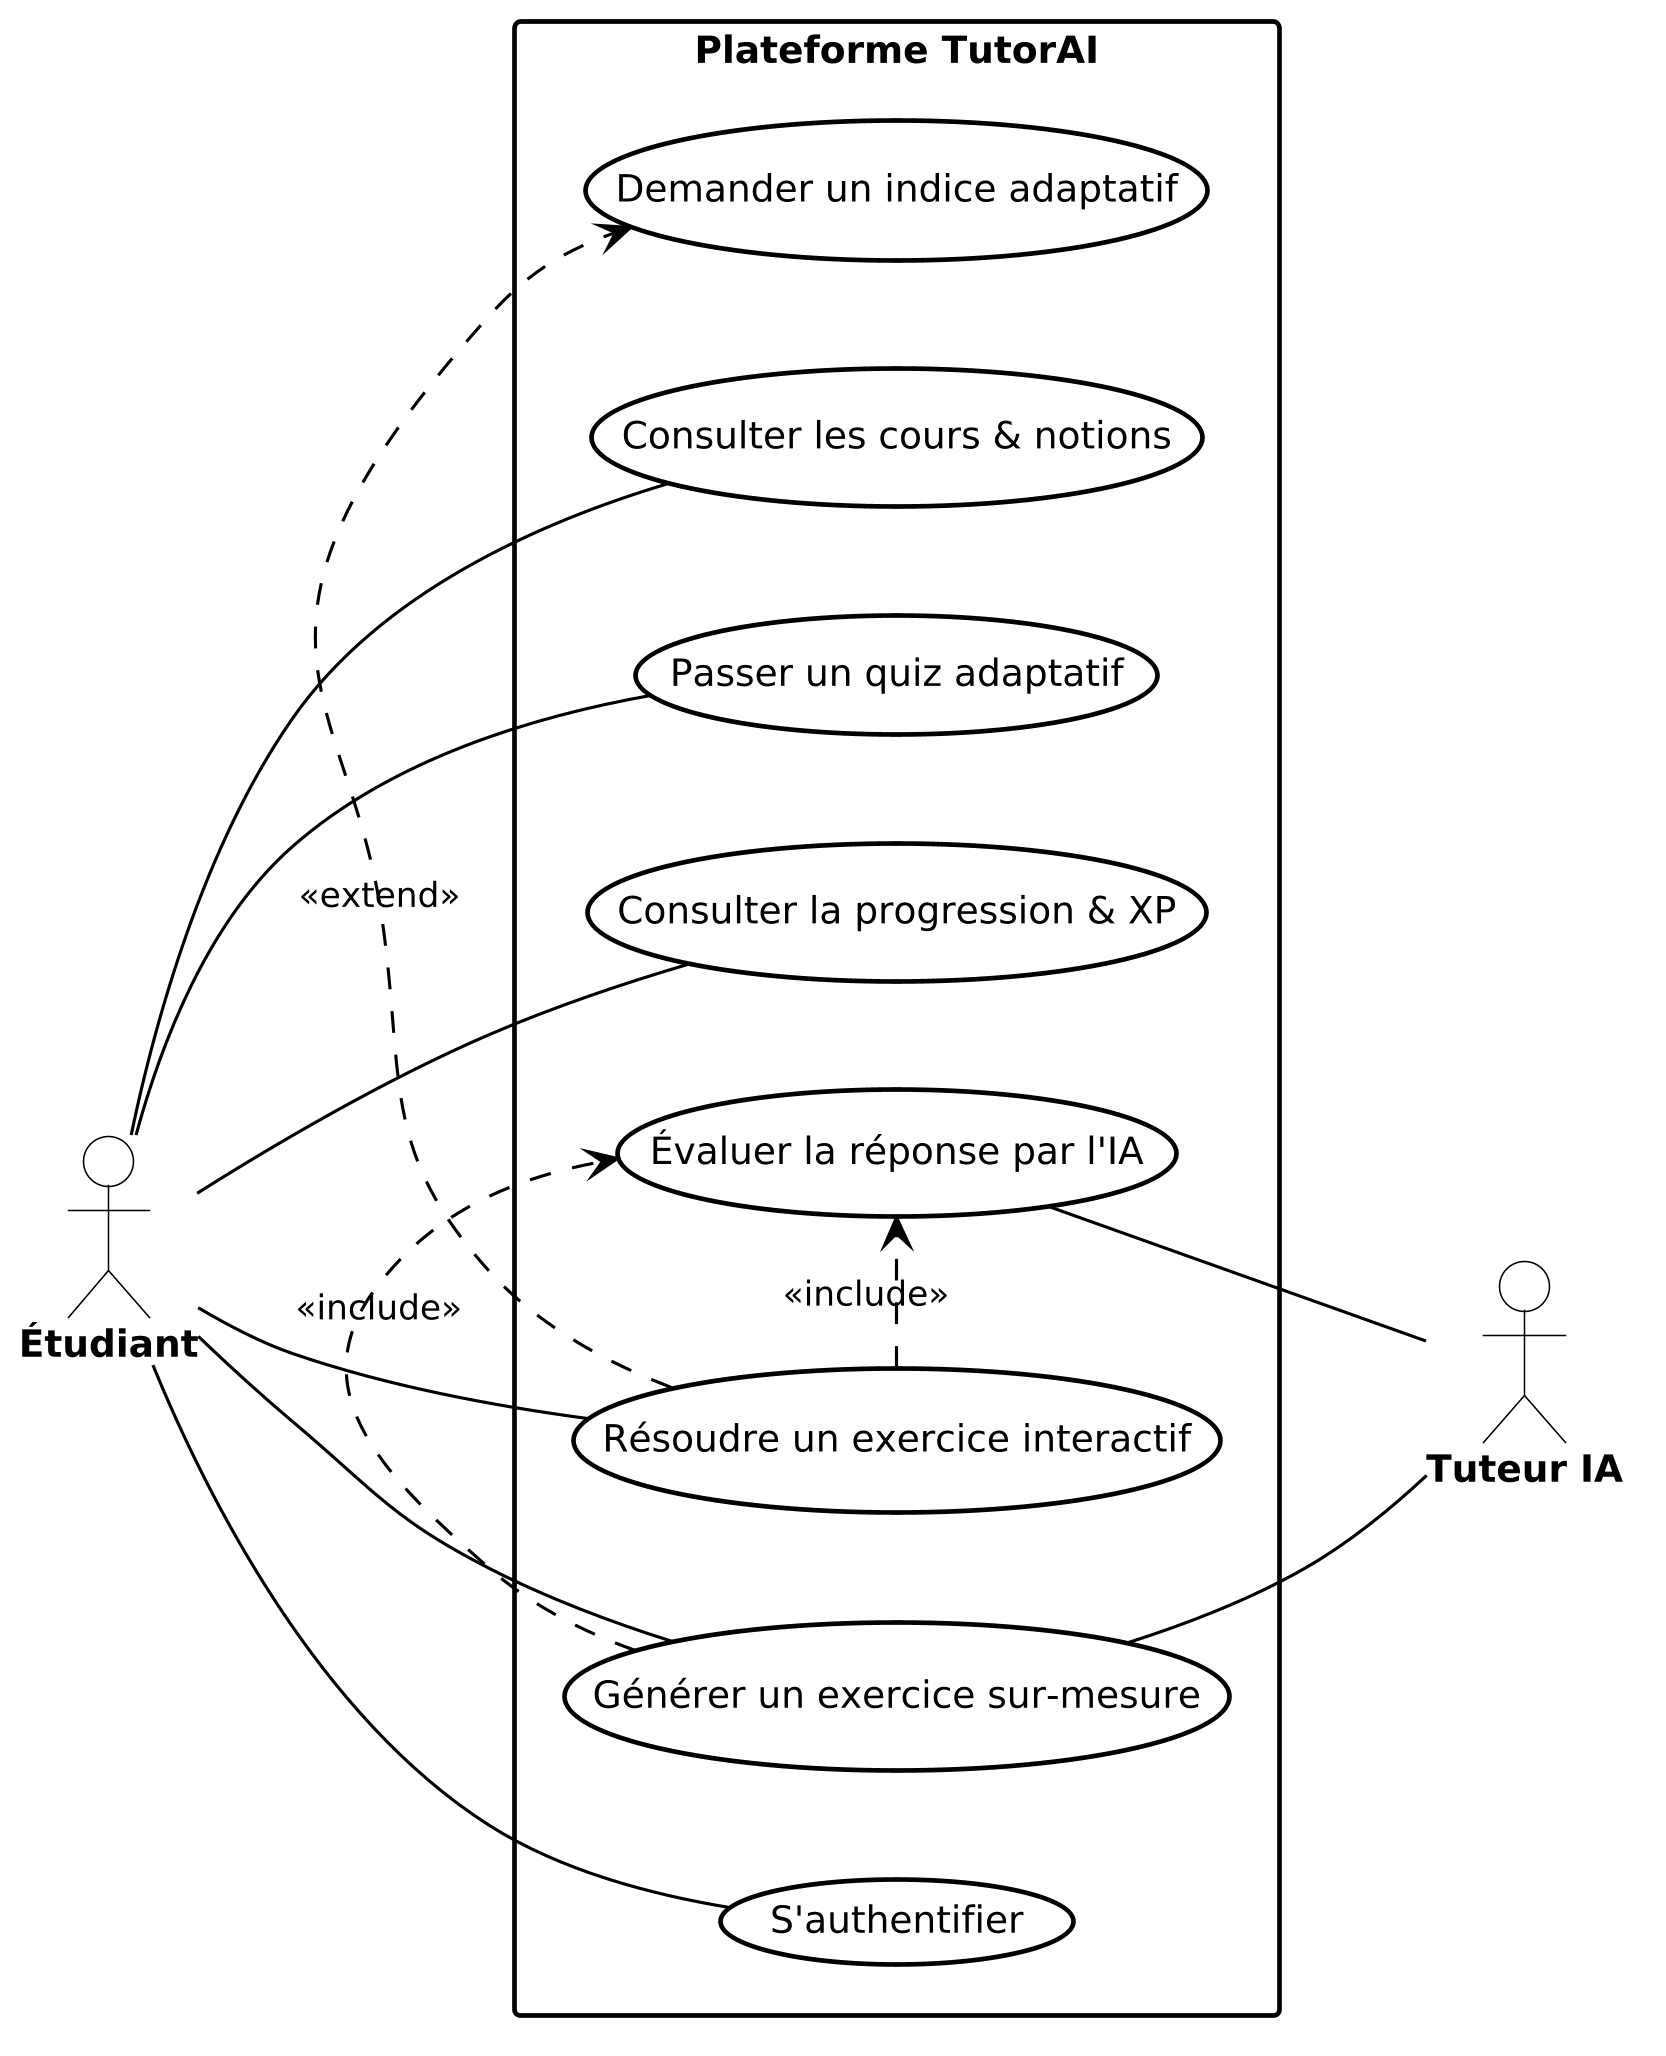
\includegraphics[width=0.95\textwidth,height=12.5cm,keepaspectratio]{use_case.png}%
  }{%
    \fbox{\parbox[c][3.5cm][c]{0.92\textwidth}{\centering
      \textbf{\large [ EMPLACEMENT PHOTO : CAS D'UTILISATION UML ]}\\[8pt]
      \small Déposez votre image dans le dossier et indiquez son nom ci-dessus :\\
      \texttt{\textbackslash includegraphics[width=0.85\textbackslash textwidth]\{use\_case.png\}}\\[6pt]
      \footnotesize\itshape Description : Diagramme global des cas d'utilisation UML (Acteurs : Étudiant, Tuteur IA).
    }}%
  }
  \caption{Diagramme global des cas d'utilisation de la plateforme TutorAI}
  \label{fig:use_case}
\end{figure}

\section{Conclusion}
Ce deuxième chapitre a permis d'établir avec précision la matrice des exigences fonctionnelles et techniques régissant la plateforme TutorAI. La formalisation des scénarios nominaux et d'exception a notamment permis de cadrer le comportement strict du moteur d'évaluation. Nous pouvons désormais aborder sereinement la phase de conception logicielle au chapitre suivant.

% ------------------------------------------------------------------------------
% CHAPITRE 3 : CONCEPTION DU SYSTÈME (PAGE 15 DU GUIDE)
% ------------------------------------------------------------------------------
\chaptercoverpage[Conception du système]{Conception\\ du système}{3}{}

\section{Introduction}
Tandis que la phase d'analyse répondait à la question « que doit faire le système ? », la phase de conception a pour vocation d'élucider « comment le réaliser techniquement ? ». Dans ce chapitre, nous détaillons la modélisation du système TutorAI sous deux angles complémentaires. D'une part, la \textbf{modélisation dynamique} retrace les interactions temporelles et comportementales (diagrammes de séquences avec fragments d'interaction UML2, diagrammes de collaboration, d'états-transitions et d'activités). D'autre part, la \textbf{modélisation statique} formalise la structure logique des données (diagramme de classes, modèle relationnel, dictionnaire de données exhaustif) ainsi que les architectures logicielle et matérielle retenues.

\section{Modélisation dynamique}
La modélisation dynamique capture la dimension temporelle de l'application et la collaboration des objets métier face aux sollicitations des utilisateurs.

\subsection{Diagrammes de séquences}
Un diagramme de séquence UML représente l'échange chronologique de messages entre objets ou lignes de vie. Conformément aux recommandations du standard UML 2, nous exploitons des messages synchrones, asynchrones ainsi que des cadres d'interaction structurants (\texttt{alt}, \texttt{opt}, \texttt{loop}).

\begin{figure}[H]
  \centering
  % >>> INSÉREZ VOTRE PHOTO ICI : Remplacez 'seq_messages.png' par le nom de votre fichier image <<<
  \IfFileExists{seq_messages.png}{%
    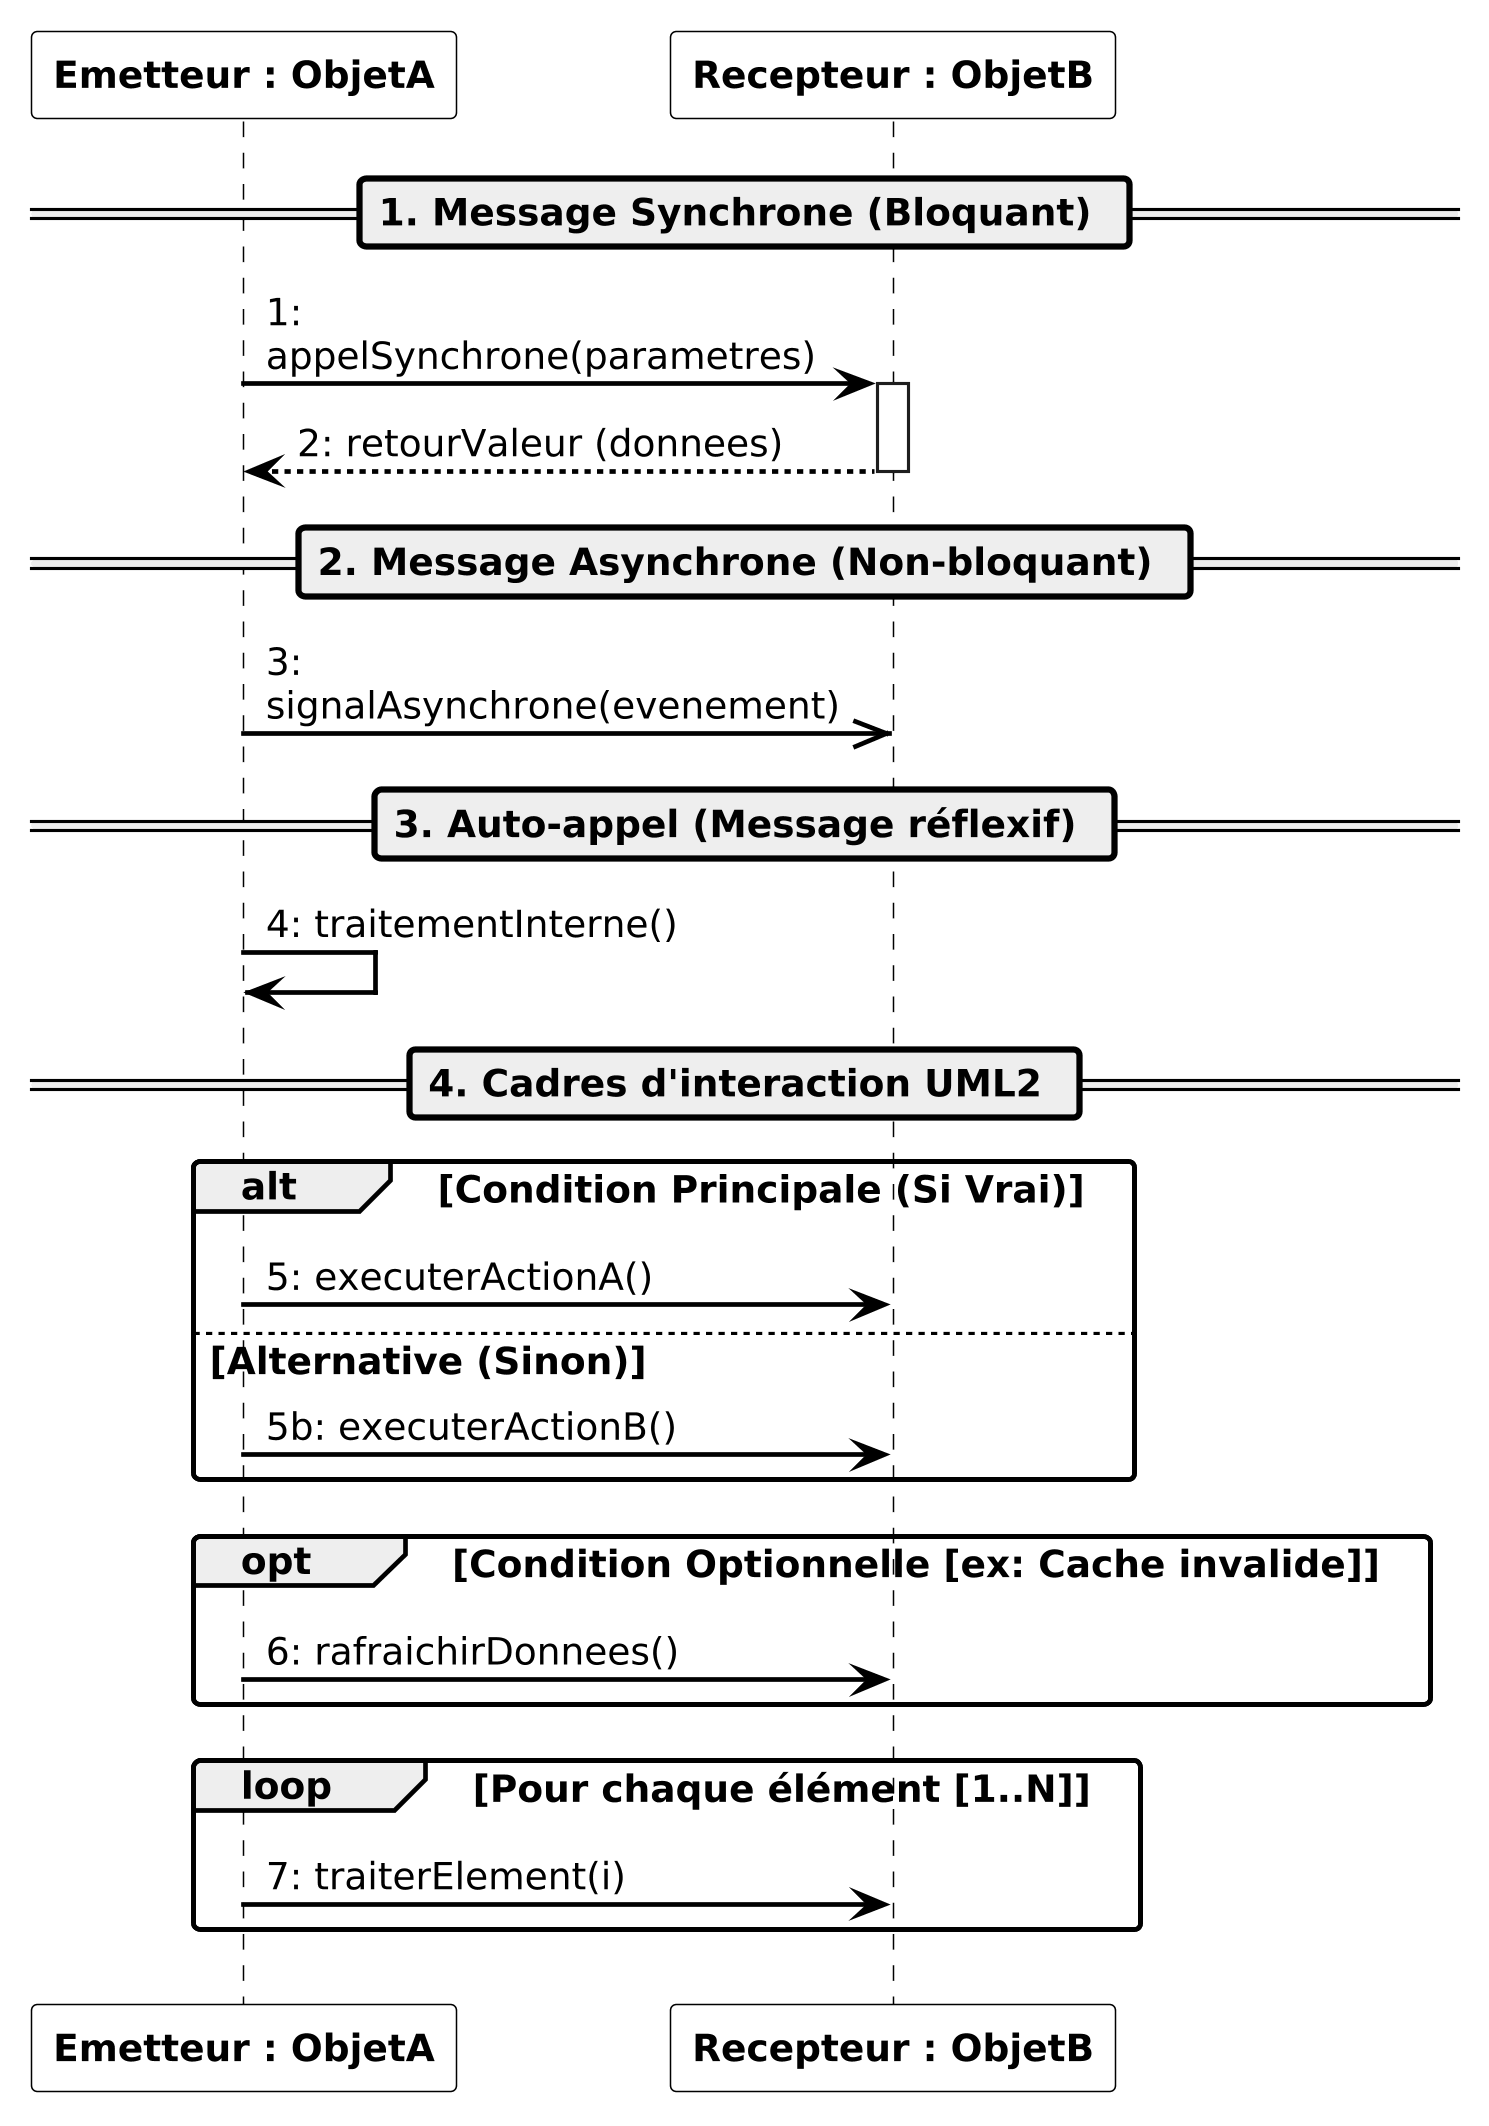
\includegraphics[width=0.95\textwidth,height=9.5cm,keepaspectratio]{seq_messages.png}%
  }{%
    \fbox{\parbox[c][3.5cm][c]{0.92\textwidth}{\centering
      \textbf{\large [ EMPLACEMENT PHOTO : TYPES DE MESSAGES SÉQUENCES ]}\\[8pt]
      \small Déposez votre image dans le dossier et indiquez son nom ci-dessus :\\
      \texttt{\textbackslash includegraphics[width=0.85\textbackslash textwidth]\{seq\_messages.png\}}\\[6pt]
      \footnotesize\itshape Description : Différents types de messages dans un diagramme de séquences UML2.
    }}%
  }
  \caption{Différents messages dans un diagramme de séquences}
  \label{fig:seq_messages}
\end{figure}

La figure \ref{fig:seq_auth} illustre le scénario d'authentification sécurisée d'un étudiant au sein de l'application :

\begin{figure}[H]
  \centering
  % >>> INSÉREZ VOTRE PHOTO ICI : Remplacez 'seq_auth.png' par le nom de votre fichier image <<<
  \IfFileExists{seq_auth.png}{%
    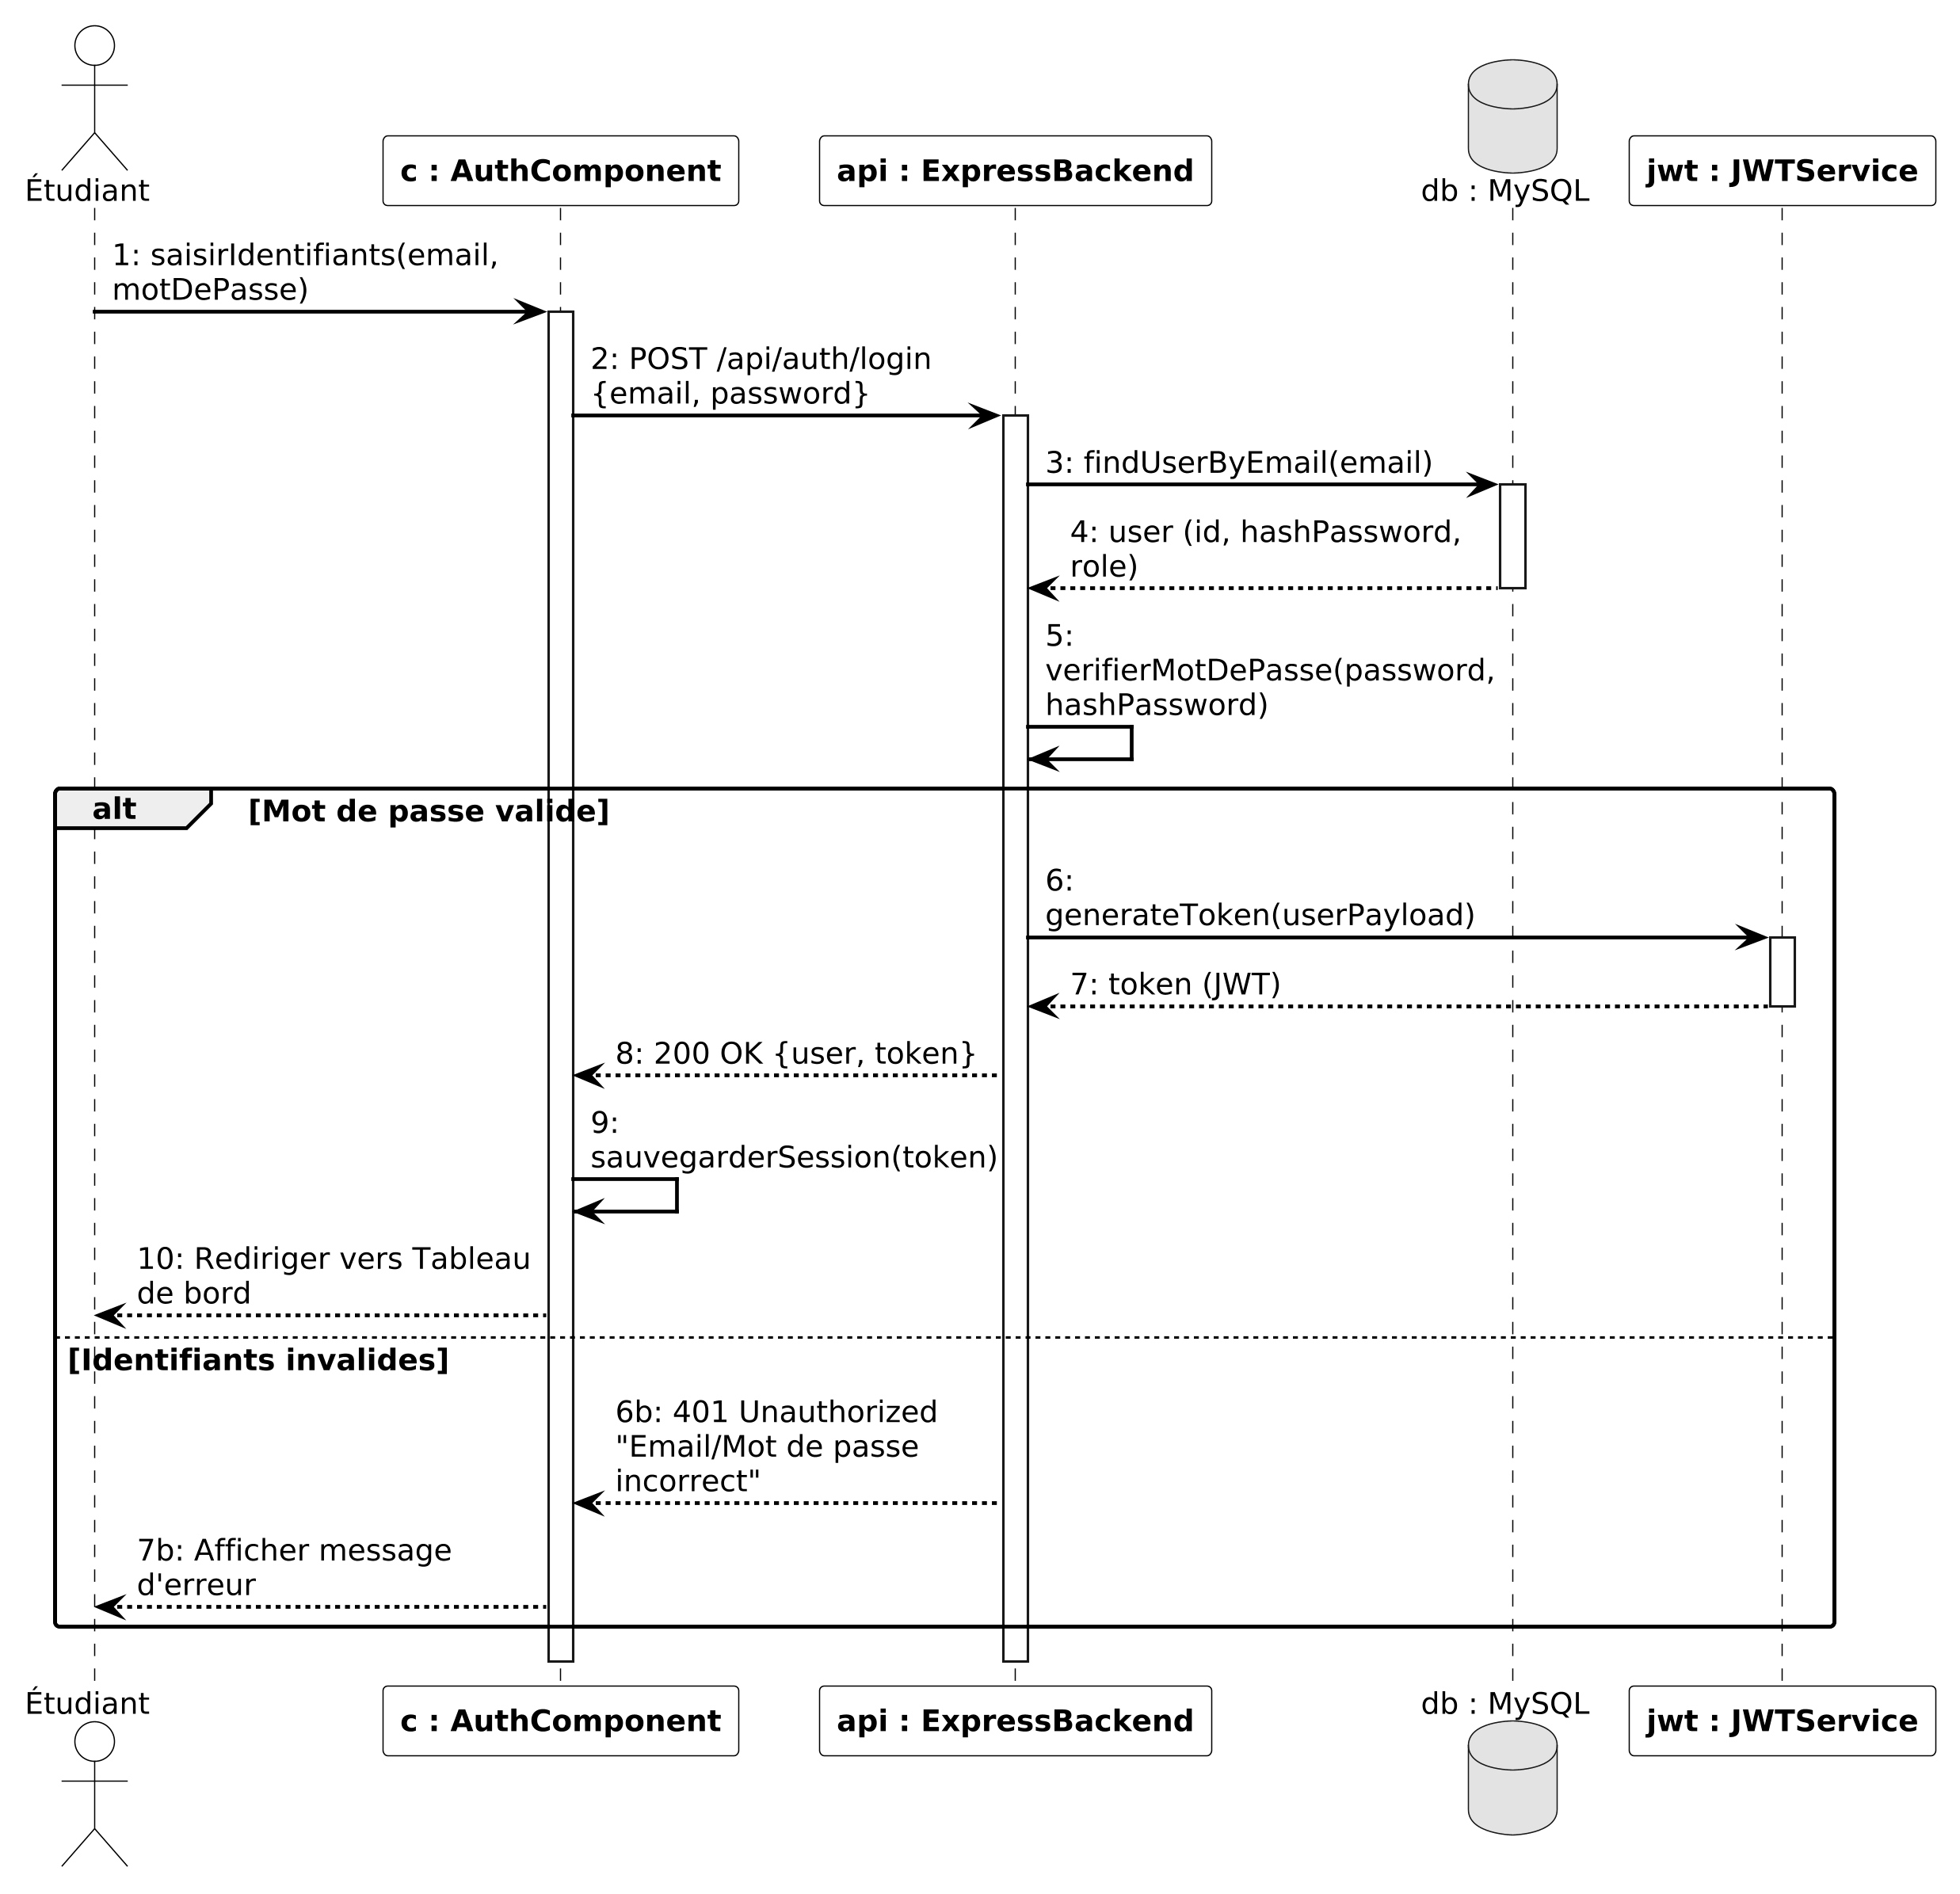
\includegraphics[width=0.95\textwidth,height=12cm,keepaspectratio]{seq_auth.png}%
  }{%
    \fbox{\parbox[c][3.5cm][c]{0.92\textwidth}{\centering
      \textbf{\large [ EMPLACEMENT PHOTO : SÉQUENCES AUTHENTIFICATION ]}\\[8pt]
      \small Déposez votre image dans le dossier et indiquez son nom ci-dessus :\\
      \texttt{\textbackslash includegraphics[width=0.85\textbackslash textwidth]\{seq\_auth.png\}}\\[6pt]
      \footnotesize\itshape Description : Diagramme de séquences UML2 du processus d'authentification (Étudiant, AuthComponent, API, MySQL, JWT).
    }}%
  }
  \caption{Diagramme de séquences "Authentification"}
  \label{fig:seq_auth}
\end{figure}

La figure \ref{fig:seq_eval} modélise l'interaction complexe entre l'interface utilisateur, le backend Express et le moteur d'inférence LLM Ollama lors de l'évaluation d'un exercice :

\begin{figure}[H]
  \centering
  % >>> INSÉREZ VOTRE PHOTO ICI : Remplacez 'seq_eval.png' par le nom de votre fichier image <<<
  \IfFileExists{seq_eval.png}{%
    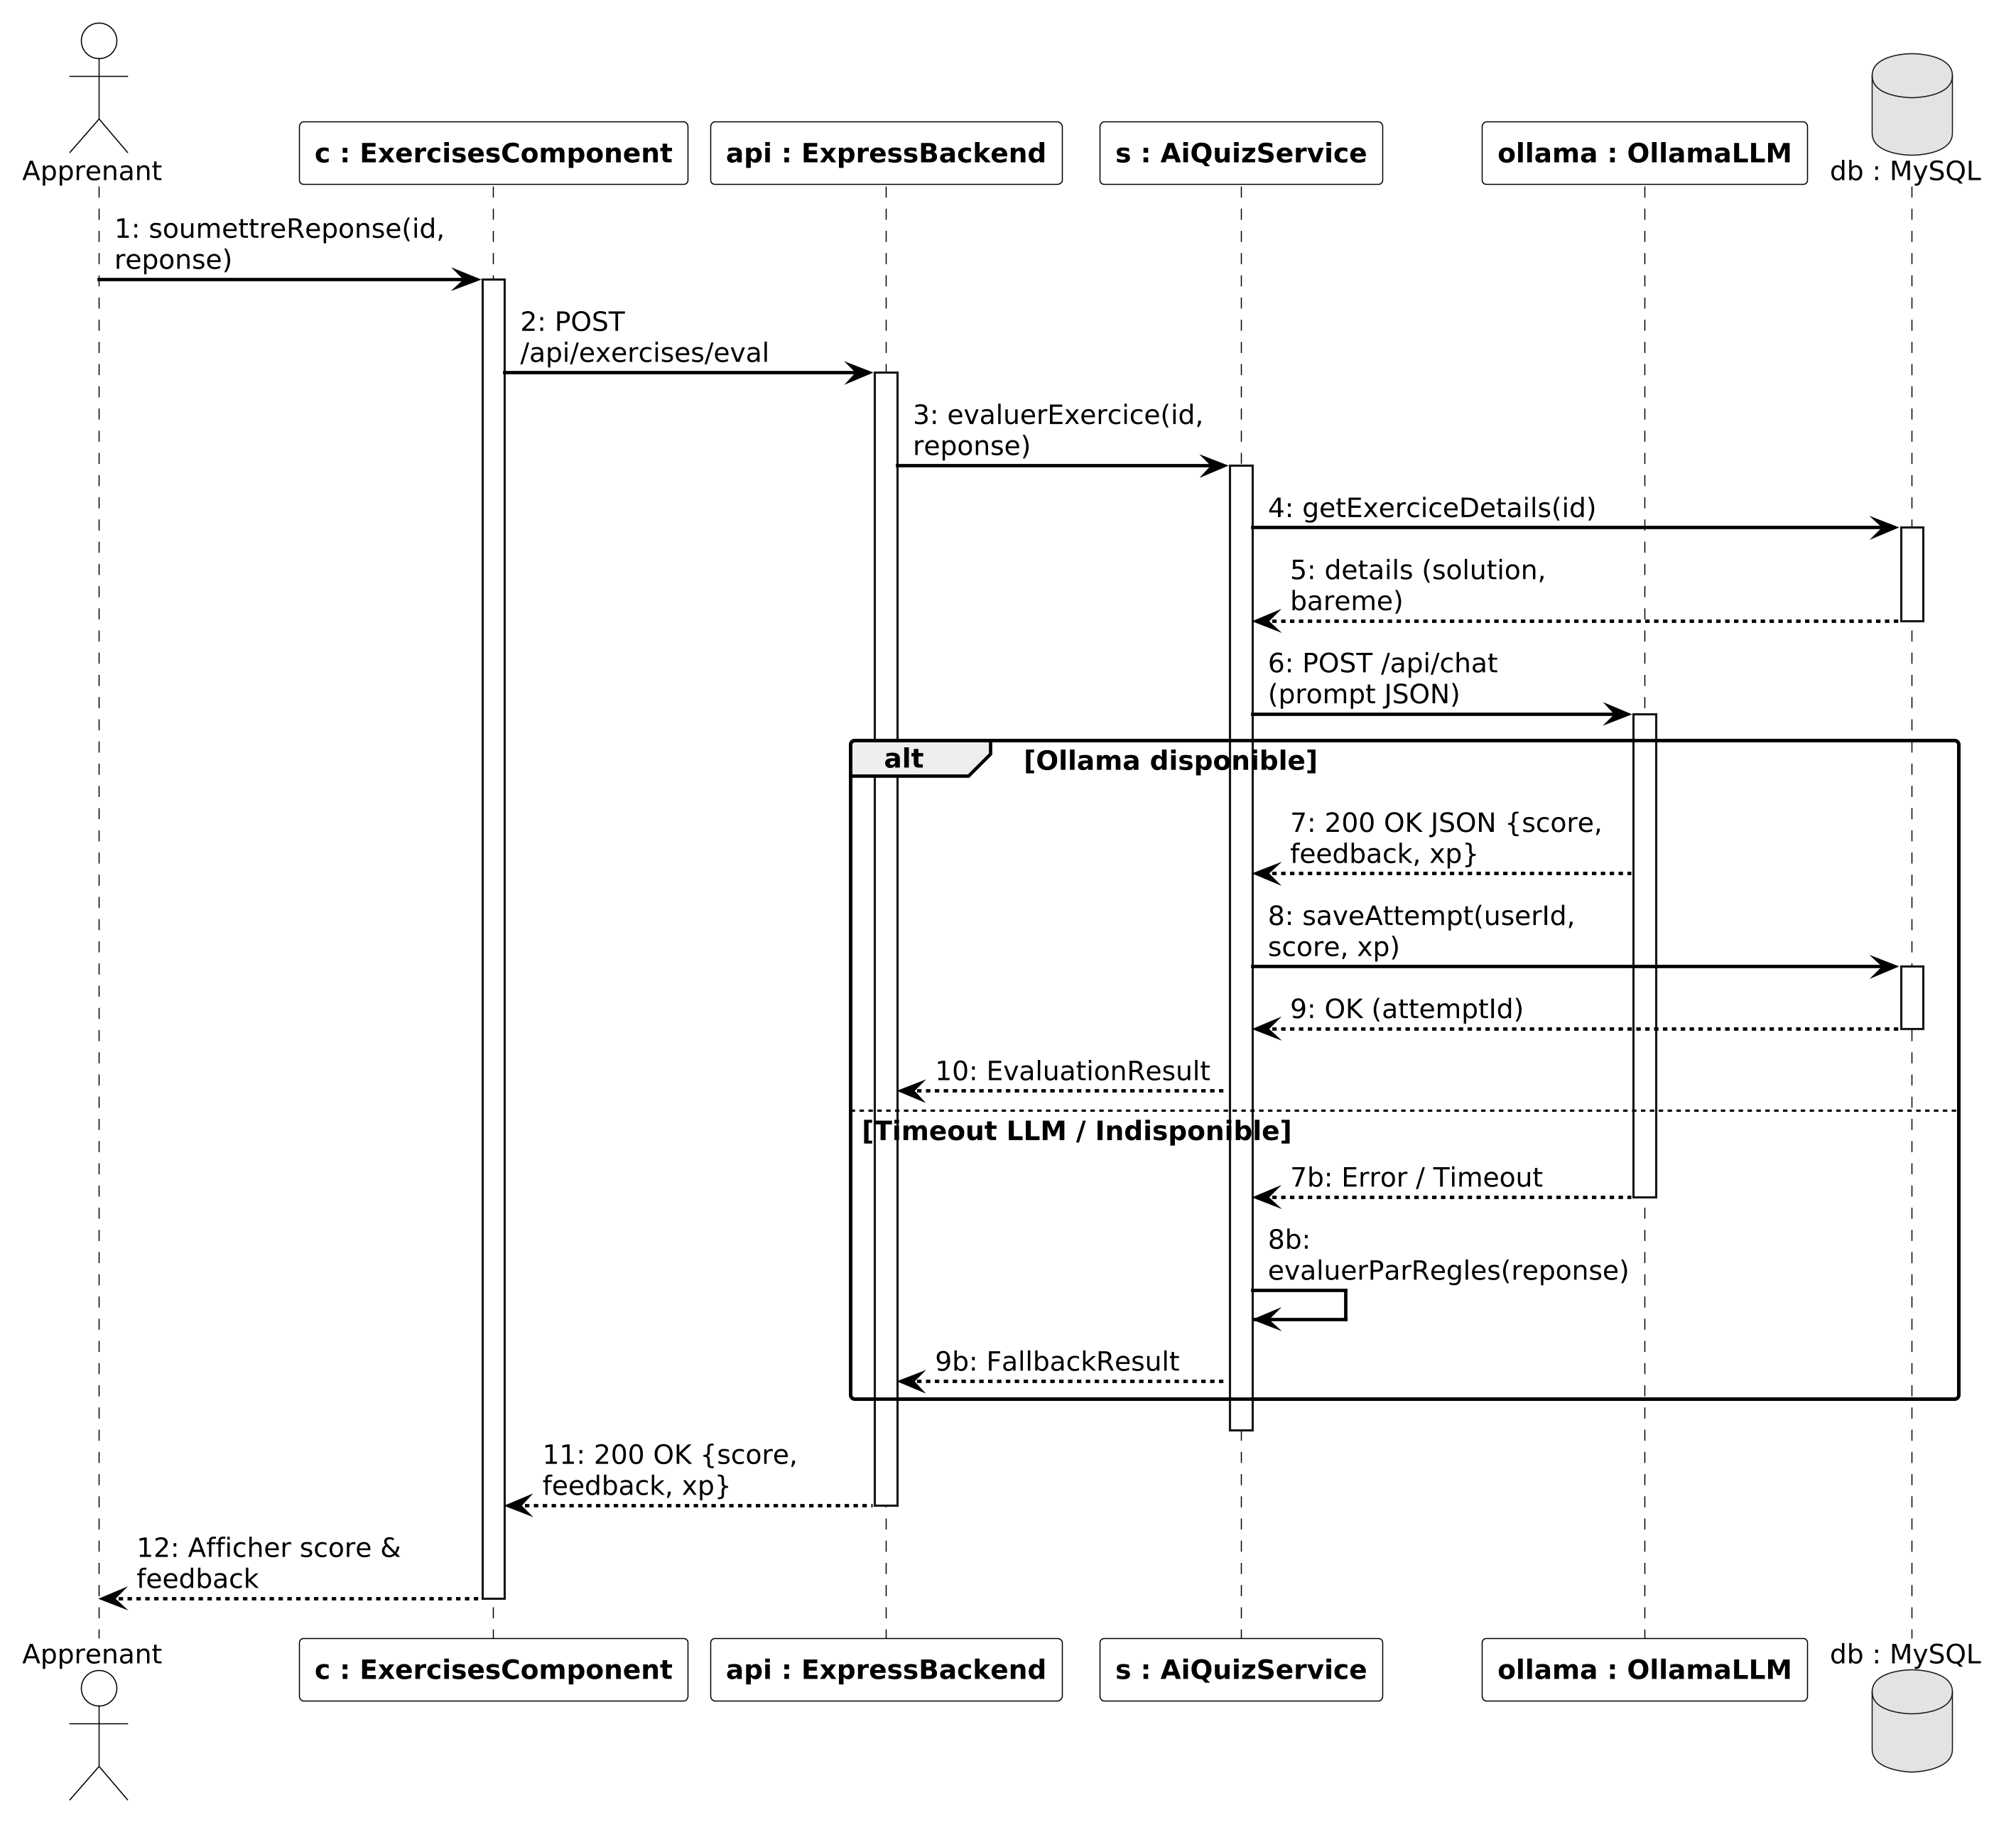
\includegraphics[width=0.95\textwidth,height=13cm,keepaspectratio]{seq_eval.png}%
  }{%
    \fbox{\parbox[c][3.5cm][c]{0.92\textwidth}{\centering
      \textbf{\large [ EMPLACEMENT PHOTO : SÉQUENCES ÉVALUATION EXERCICE ]}\\[8pt]
      \small Déposez votre image dans le dossier et indiquez son nom ci-dessus :\\
      \texttt{\textbackslash includegraphics[width=0.85\textbackslash textwidth]\{seq\_eval.png\}}\\[6pt]
      \footnotesize\itshape Description : Diagramme de séquences UML2 de l'évaluation rigoureuse d'un exercice.
    }}%
  }
  \caption{Diagramme de séquences de l'évaluation rigoureuse d'un exercice}
  \label{fig:seq_eval}
\end{figure}

\subsection{Diagrammes de collaboration}
Le diagramme de collaboration met l'accent sur l'organisation spatiale des objets et la topologie des liens qui les unissent. Dans TutorAI, le composant d'orchestration pédagogique (\texttt{AiLearningService}) communique directement avec les services de persistance locale, le gestionnaire de session et le client HTTP Angular.

\begin{figure}[H]
  \centering
  % >>> INSÉREZ VOTRE PHOTO ICI : Remplacez 'collab.png' par le nom de votre fichier image <<<
  \IfFileExists{collab.png}{%
    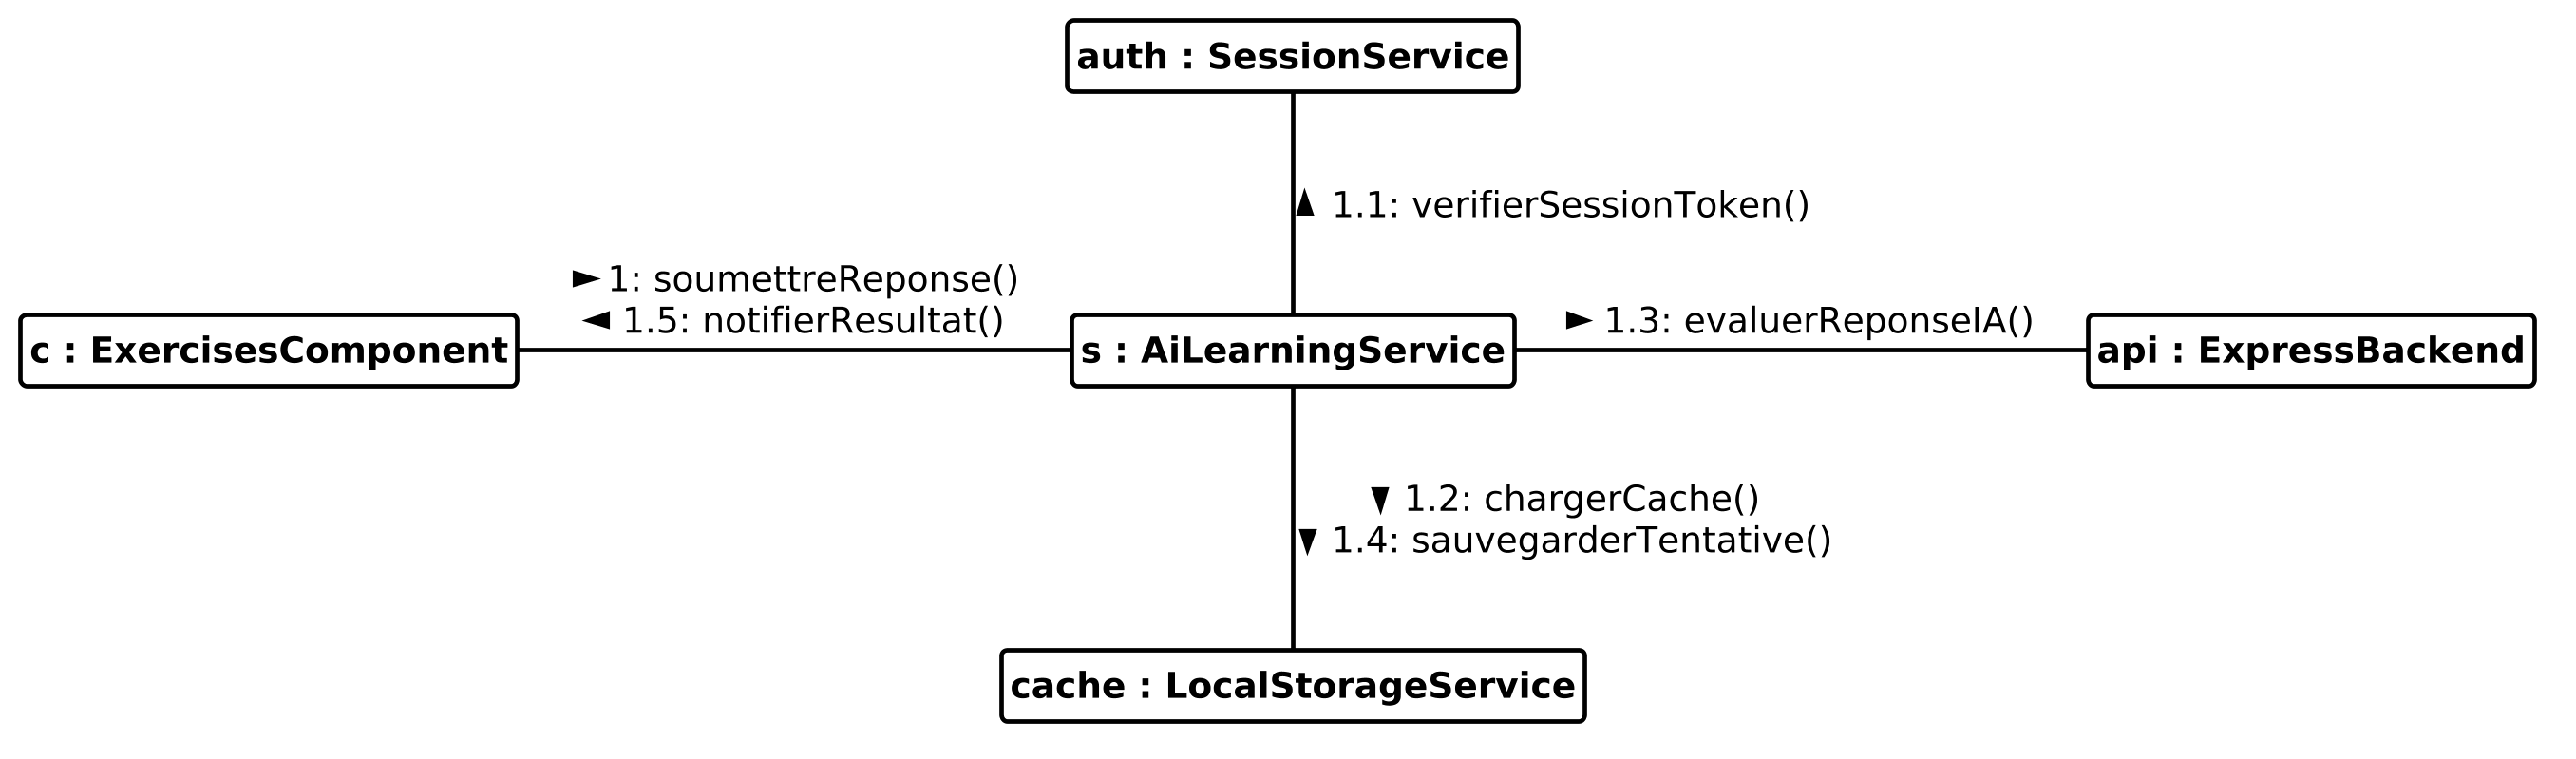
\includegraphics[width=0.95\textwidth,height=11cm,keepaspectratio]{collab.png}%
  }{%
    \fbox{\parbox[c][3.5cm][c]{0.92\textwidth}{\centering
      \textbf{\large [ EMPLACEMENT PHOTO : DIAGRAMME DE COLLABORATION ]}\\[8pt]
      \small Déposez votre image dans le dossier et indiquez son nom ci-dessus :\\
      \texttt{\textbackslash includegraphics[width=0.85\textbackslash textwidth]\{collab.png\}}\\[6pt]
      \footnotesize\itshape Description : Diagramme de collaboration entre les services du sous-système de tutorat.
    }}%
  }
  \caption{Diagramme de collaboration entre les services du sous-système de tutorat}
  \label{fig:collab}
\end{figure}

\subsection{Diagrammes d'états}
Les diagrammes d'états décrivent les différents états stables qu'une entité du système peut adopter au cours de son existence sous l'action d'événements déclencheurs.

\subsection{Diagrammes d'état-transition}
Le comportement interne d'un exercice pratique au sein d'une session d'apprentissage est régit par l'automate à états finis représenté sur la figure \ref{fig:state_machine}.

\begin{figure}[H]
  \centering
  % >>> INSÉREZ VOTRE PHOTO ICI : Remplacez 'state_machine.png' par le nom de votre fichier image <<<
  \IfFileExists{state_machine.png}{%
    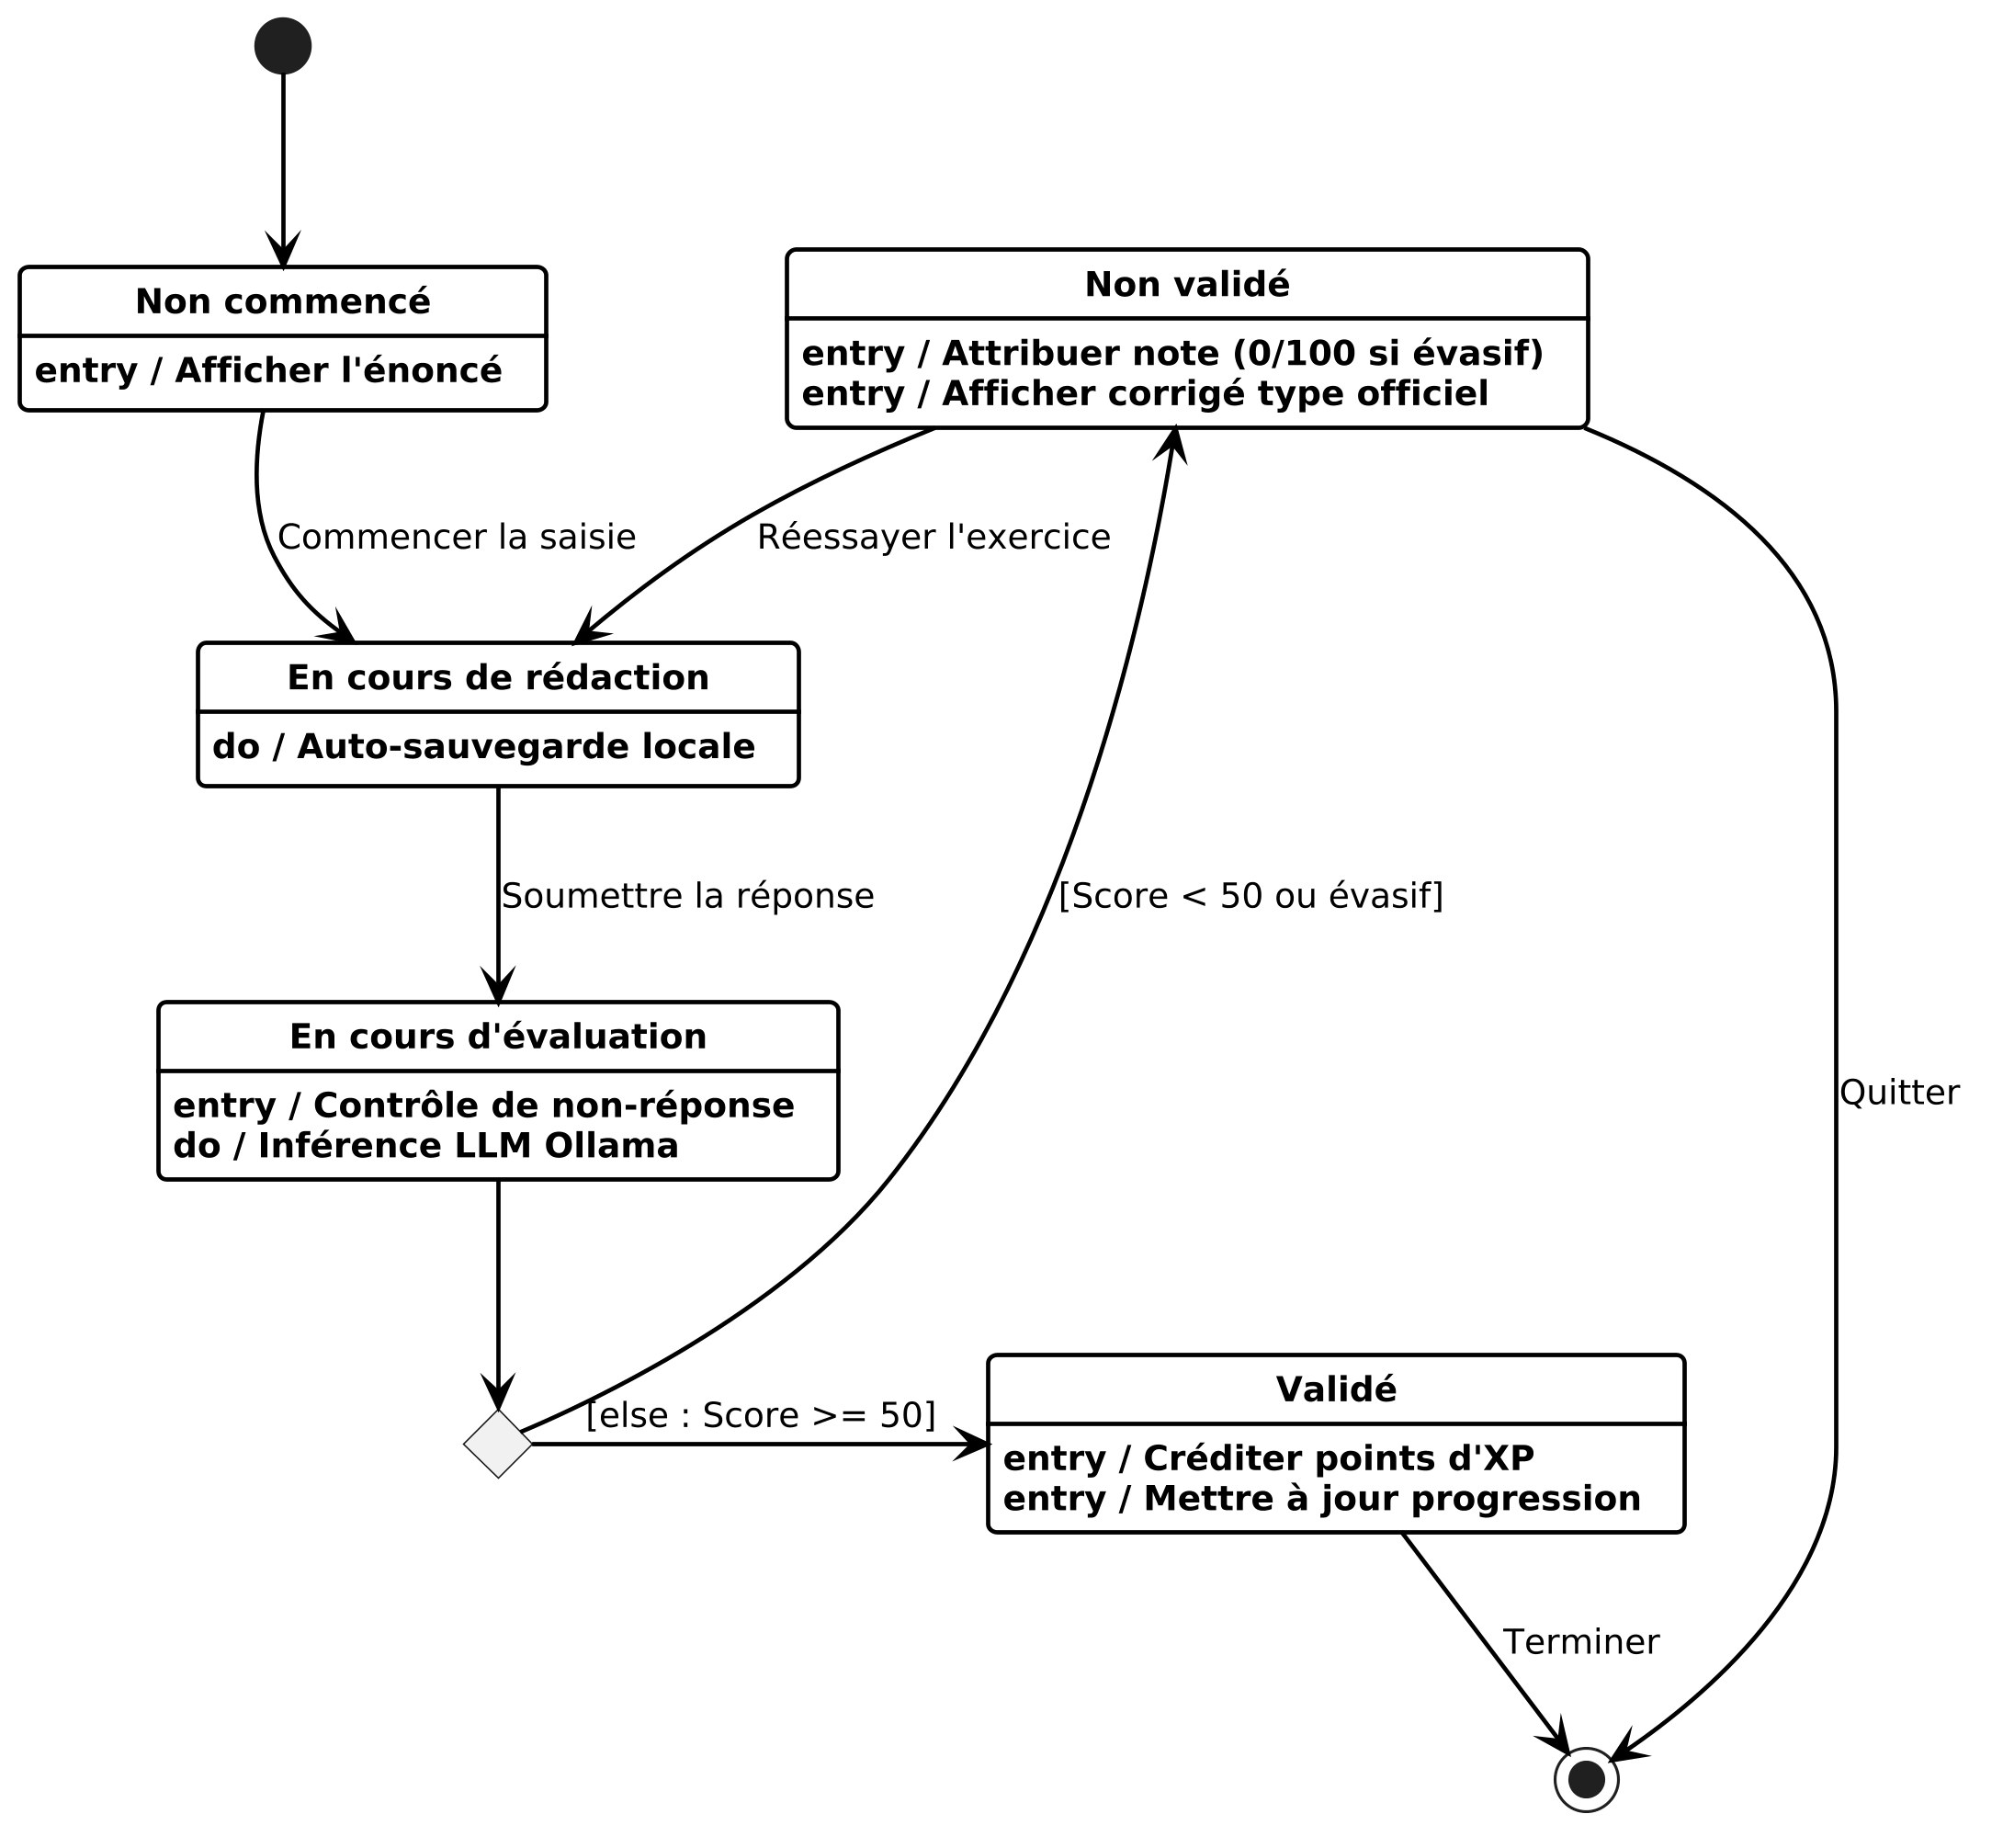
\includegraphics[width=0.95\textwidth,height=10.5cm,keepaspectratio]{state_machine.png}%
  }{%
    \fbox{\parbox[c][3.5cm][c]{0.92\textwidth}{\centering
      \textbf{\large [ EMPLACEMENT PHOTO : DIAGRAMME D'ÉTAT-TRANSITION ]}\\[8pt]
      \small Déposez votre image dans le dossier et indiquez son nom ci-dessus :\\
      \texttt{\textbackslash includegraphics[width=0.85\textbackslash textwidth]\{state\_machine.png\}}\\[6pt]
      \footnotesize\itshape Description : Diagramme d'états-transitions du cycle de vie d'un exercice pratique.
    }}%
  }
  \caption{Diagramme d'état-transition du cycle de vie d'un exercice}
  \label{fig:state_machine}
\end{figure}

\subsection{Diagrammes d'activité}
Le diagramme d'activité de la figure \ref{fig:activity} détaille le flot de contrôle logique lors de la soumission d'une réponse d'exercice, matérialisant le routage vers l'intercepteur de non-réponses ou vers le serveur d'inférence LLM.

\begin{figure}[H]
  \centering
  % >>> INSÉREZ VOTRE PHOTO ICI : Remplacez 'activity.png' par le nom de votre fichier image <<<
  \IfFileExists{activity.png}{%
    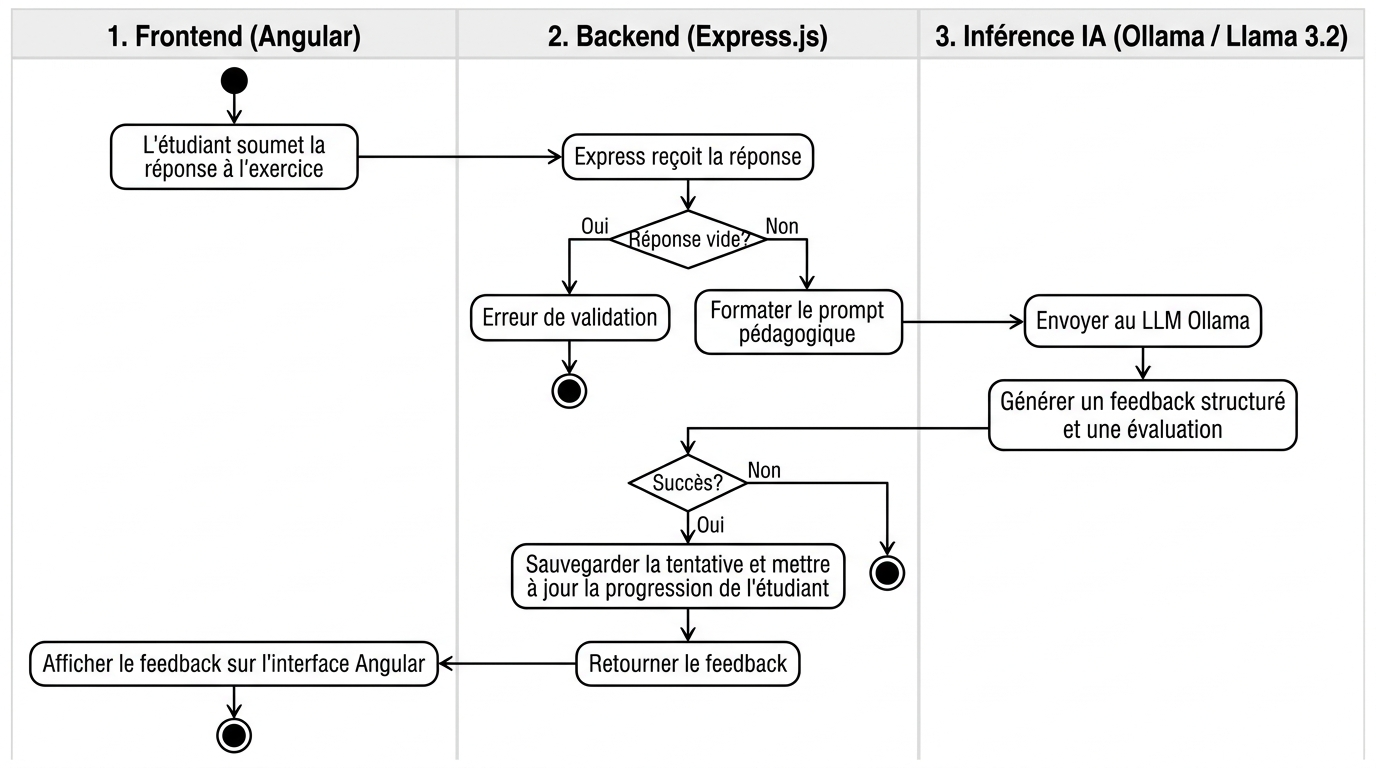
\includegraphics[width=0.95\textwidth,height=18cm,keepaspectratio]{activity.png}%
  }{%
    \fbox{\parbox[c][3.5cm][c]{0.92\textwidth}{\centering
      \textbf{\large [ EMPLACEMENT PHOTO : DIAGRAMME D'ACTIVITÉS ]}\\[8pt]
      \small Déposez votre image dans le dossier et indiquez son nom ci-dessus :\\
      \texttt{\textbackslash includegraphics[width=0.85\textbackslash textwidth]\{activity.png\}}\\[6pt]
      \footnotesize\itshape Description : Diagramme d'activités UML du processus d'évaluation adaptative.
    }}%
  }
  \caption{Diagramme d'activité de l'évaluation adaptative}
  \label{fig:activity}
\end{figure}

\section{Modélisation statique}
La modélisation statique formalise la structure des entités logicielles et persistantes composant la plateforme TutorAI.

\subsection{Diagramme de classes}
La structure orientée objet repose sur des entités fortement typées représentant l'étudiant, son profil diagnostique, ses résultats de quiz et la hiérarchie des exercices pratiques. La figure \ref{fig:class_diag} schématise les classes principales et leurs relations.

\begin{figure}[H]
  \centering
  % >>> INSÉREZ VOTRE PHOTO ICI : Remplacez 'class_diag.png' par le nom de votre fichier image <<<
  \IfFileExists{class_diag.png}{%
    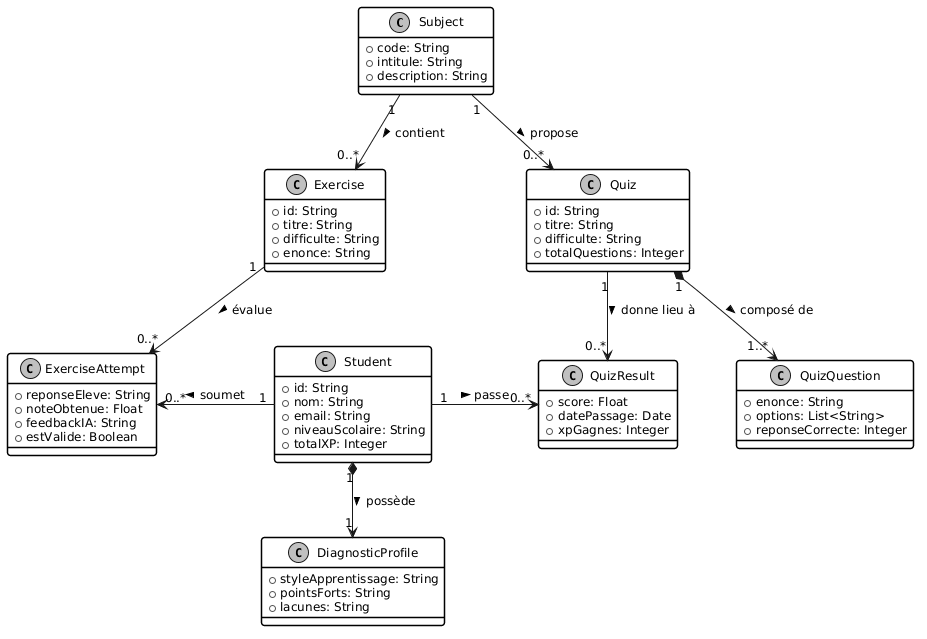
\includegraphics[width=0.95\textwidth,height=12cm,keepaspectratio]{class_diag.png}%
  }{%
    \fbox{\parbox[c][3.5cm][c]{0.92\textwidth}{\centering
      \textbf{\large [ EMPLACEMENT PHOTO : DIAGRAMME DE CLASSES ]}\\[8pt]
      \small Déposez votre image dans le dossier et indiquez son nom ci-dessus :\\
      \texttt{\textbackslash includegraphics[width=0.85\textbackslash textwidth]\{class\_diag.png\}}\\[6pt]
      \footnotesize\itshape Description : Diagramme de classes UML du domaine TutorAI.
    }}%
  }
  \caption{Diagramme de classes du domaine TutorAI}
  \label{fig:class_diag}
\end{figure}

\subsection{Modèle relationnel}
La transition du diagramme de classes vers le modèle relationnel obéit aux règles de passage fondamentales de la modélisation des données :
\begin{enumerate}
  \item Toute classe se transforme en relation (table), dont les attributs deviennent les colonnes,
  \item Tout identifiant unique devient clé primaire soulignée (\underline{clé}),
  \item Pour une association 1 à plusieurs ($1..*$), la clé primaire de la table côté 1 migre en clé étrangère (\#clé) dans la table côté $N$.
\end{enumerate}

Le schéma relationnel obtenu en troisième forme normale (3FN) s'exprime comme suit :
\begin{itemize}
  \item[—] \textbf{STUDENTS} (\underline{id}, email, password\_hash, first\_name, education\_level, created\_at),
  \item[—] \textbf{LEARNING\_PROFILES} (\underline{id}, \#student\_id, current\_subject, total\_xp, learning\_preferences,\\
  \hspace*{0.5cm}updated\_at),
  \item[—] \textbf{DIFFICULTIES} (\underline{id}, \#student\_id, difficulty, created\_at),
  \item[—] \textbf{DIAGNOSTIC\_RESULTS} (\underline{id}, \#student\_id, score, strengths, weaknesses, created\_at),
  \item[—] \textbf{SUBJECT\_PROGRESS} (\underline{id}, \#student\_id, subject, quizzes\_completed, exercises\_completed,\\
  \hspace*{0.5cm}average\_score, mastery\_level, adaptive\_difficulty, level\_index, updated\_at),
  \item[—] \textbf{SAVED\_EXERCISES} (\underline{id}, \#student\_id, subject, exercise\_data, completed, score, created\_at).
\end{itemize}

\subsection{Dictionnaire de données}
Le tableau \ref{tab:dict_donnees} détaille la structure et les contraintes d'intégrité appliquées aux champs de la base relationnelle MySQL.

\begin{table}[H]
\centering
\caption{Dictionnaire de données}
\label{tab:dict_donnees}
\resizebox{\textwidth}{!}{%
\begin{tabular}{|l|c|c|c|c|c|c|c|l|}
\hline
\rowcolor{LightGray}
\textbf{Nom de la colonne} & \textbf{Type de données} & \textbf{Taille} & \textbf{Obligatoire (Oui/Non)} & \textbf{Valeur par défaut} & \textbf{Valeurs autorisées} & \textbf{Clé Primaire} & \textbf{Clé Étrangère} & \textbf{Nom de la Table} \\ \hline
id & VARCHAR & 36 & Oui & UUID() & Chaîne hexadécimale & Oui & Non & students \\ \hline
email & VARCHAR & 255 & Oui & NULL & Format email unique & Non & Non & students \\ \hline
password\_hash & VARCHAR & 255 & Oui & NULL & Chaîne hachée BCrypt & Non & Non & students \\ \hline
first\_name & VARCHAR & 100 & Non & NULL & Texte alphabétique & Non & Non & students \\ \hline
education\_level & VARCHAR & 100 & Non & Lycée & Lycée, Supérieur, Univ & Non & Non & students \\ \hline
created\_at & DATETIME & -- & Oui & CURRENT & Format timestamp & Non & Non & students \\ \hline
id & VARCHAR & 36 & Oui & UUID() & Chaîne hexadécimale & Oui & Non & subject\_progress \\ \hline
student\_id & VARCHAR & 36 & Oui & NULL & Clé référençant students & Non & Oui & subject\_progress \\ \hline
subject & VARCHAR & 100 & Oui & NULL & Liste matières autorisées & Non & Non & subject\_progress \\ \hline
quizzes\_completed & INT & -- & Oui & 0 & Entier positif $\ge 0$ & Non & Non & subject\_progress \\ \hline
exercises\_completed & INT & -- & Oui & 0 & Entier positif $\ge 0$ & Non & Non & subject\_progress \\ \hline
average\_score & DECIMAL & 5,2 & Oui & 0.00 & Intervalle $[0.00 ; 100.00]$ & Non & Non & subject\_progress \\ \hline
adaptive\_difficulty & VARCHAR & 50 & Oui & Débutant & Débutant, Interm., Avancé & Non & Non & subject\_progress \\ \hline
level\_index & INT & -- & Oui & 1 & 1, 2 ou 3 & Non & Non & subject\_progress \\ \hline
\end{tabular}%
}
\end{table}

\subsection{Architecture de l'application}

\subsubsection{Architecture logiciel}
L'application repose sur une architecture moderne à trois niveaux (\textbf{3-Tiers}) garantissant la séparation étanche des responsabilités :
\begin{itemize}
  \item[—] \textbf{Couche Présentation (Front-End) :} Single Page Application développée sous Angular 16, articulée autour de composants autonomes (\textit{Standalone Components}), de services injectables réactifs basés sur RxJS et de directives d'affichage,
  \item[—] \textbf{Couche Métier et Services (Back-End) :} Serveur Node.js avec Express 5 exposant des API RESTful modulaires. Il gère l'orchestration des données, la validation des règles de gestion, la sécurisation des sessions et la communication avec le serveur d'inférence,
  \item[—] \textbf{Couche Données et Inférence (Persistance \& IA) :} Système MySQL 8 pour le stockage relationnel et moteur Ollama (Llama 3.2) encapsulé dans un environnement local pour l'évaluation et la génération dynamique.
\end{itemize}

\begin{figure}[H]
  \centering
  % >>> INSÉREZ VOTRE PHOTO ICI : Remplacez 'comp_diag.png' par le nom de votre fichier image <<<
  \IfFileExists{comp_diag.png}{%
    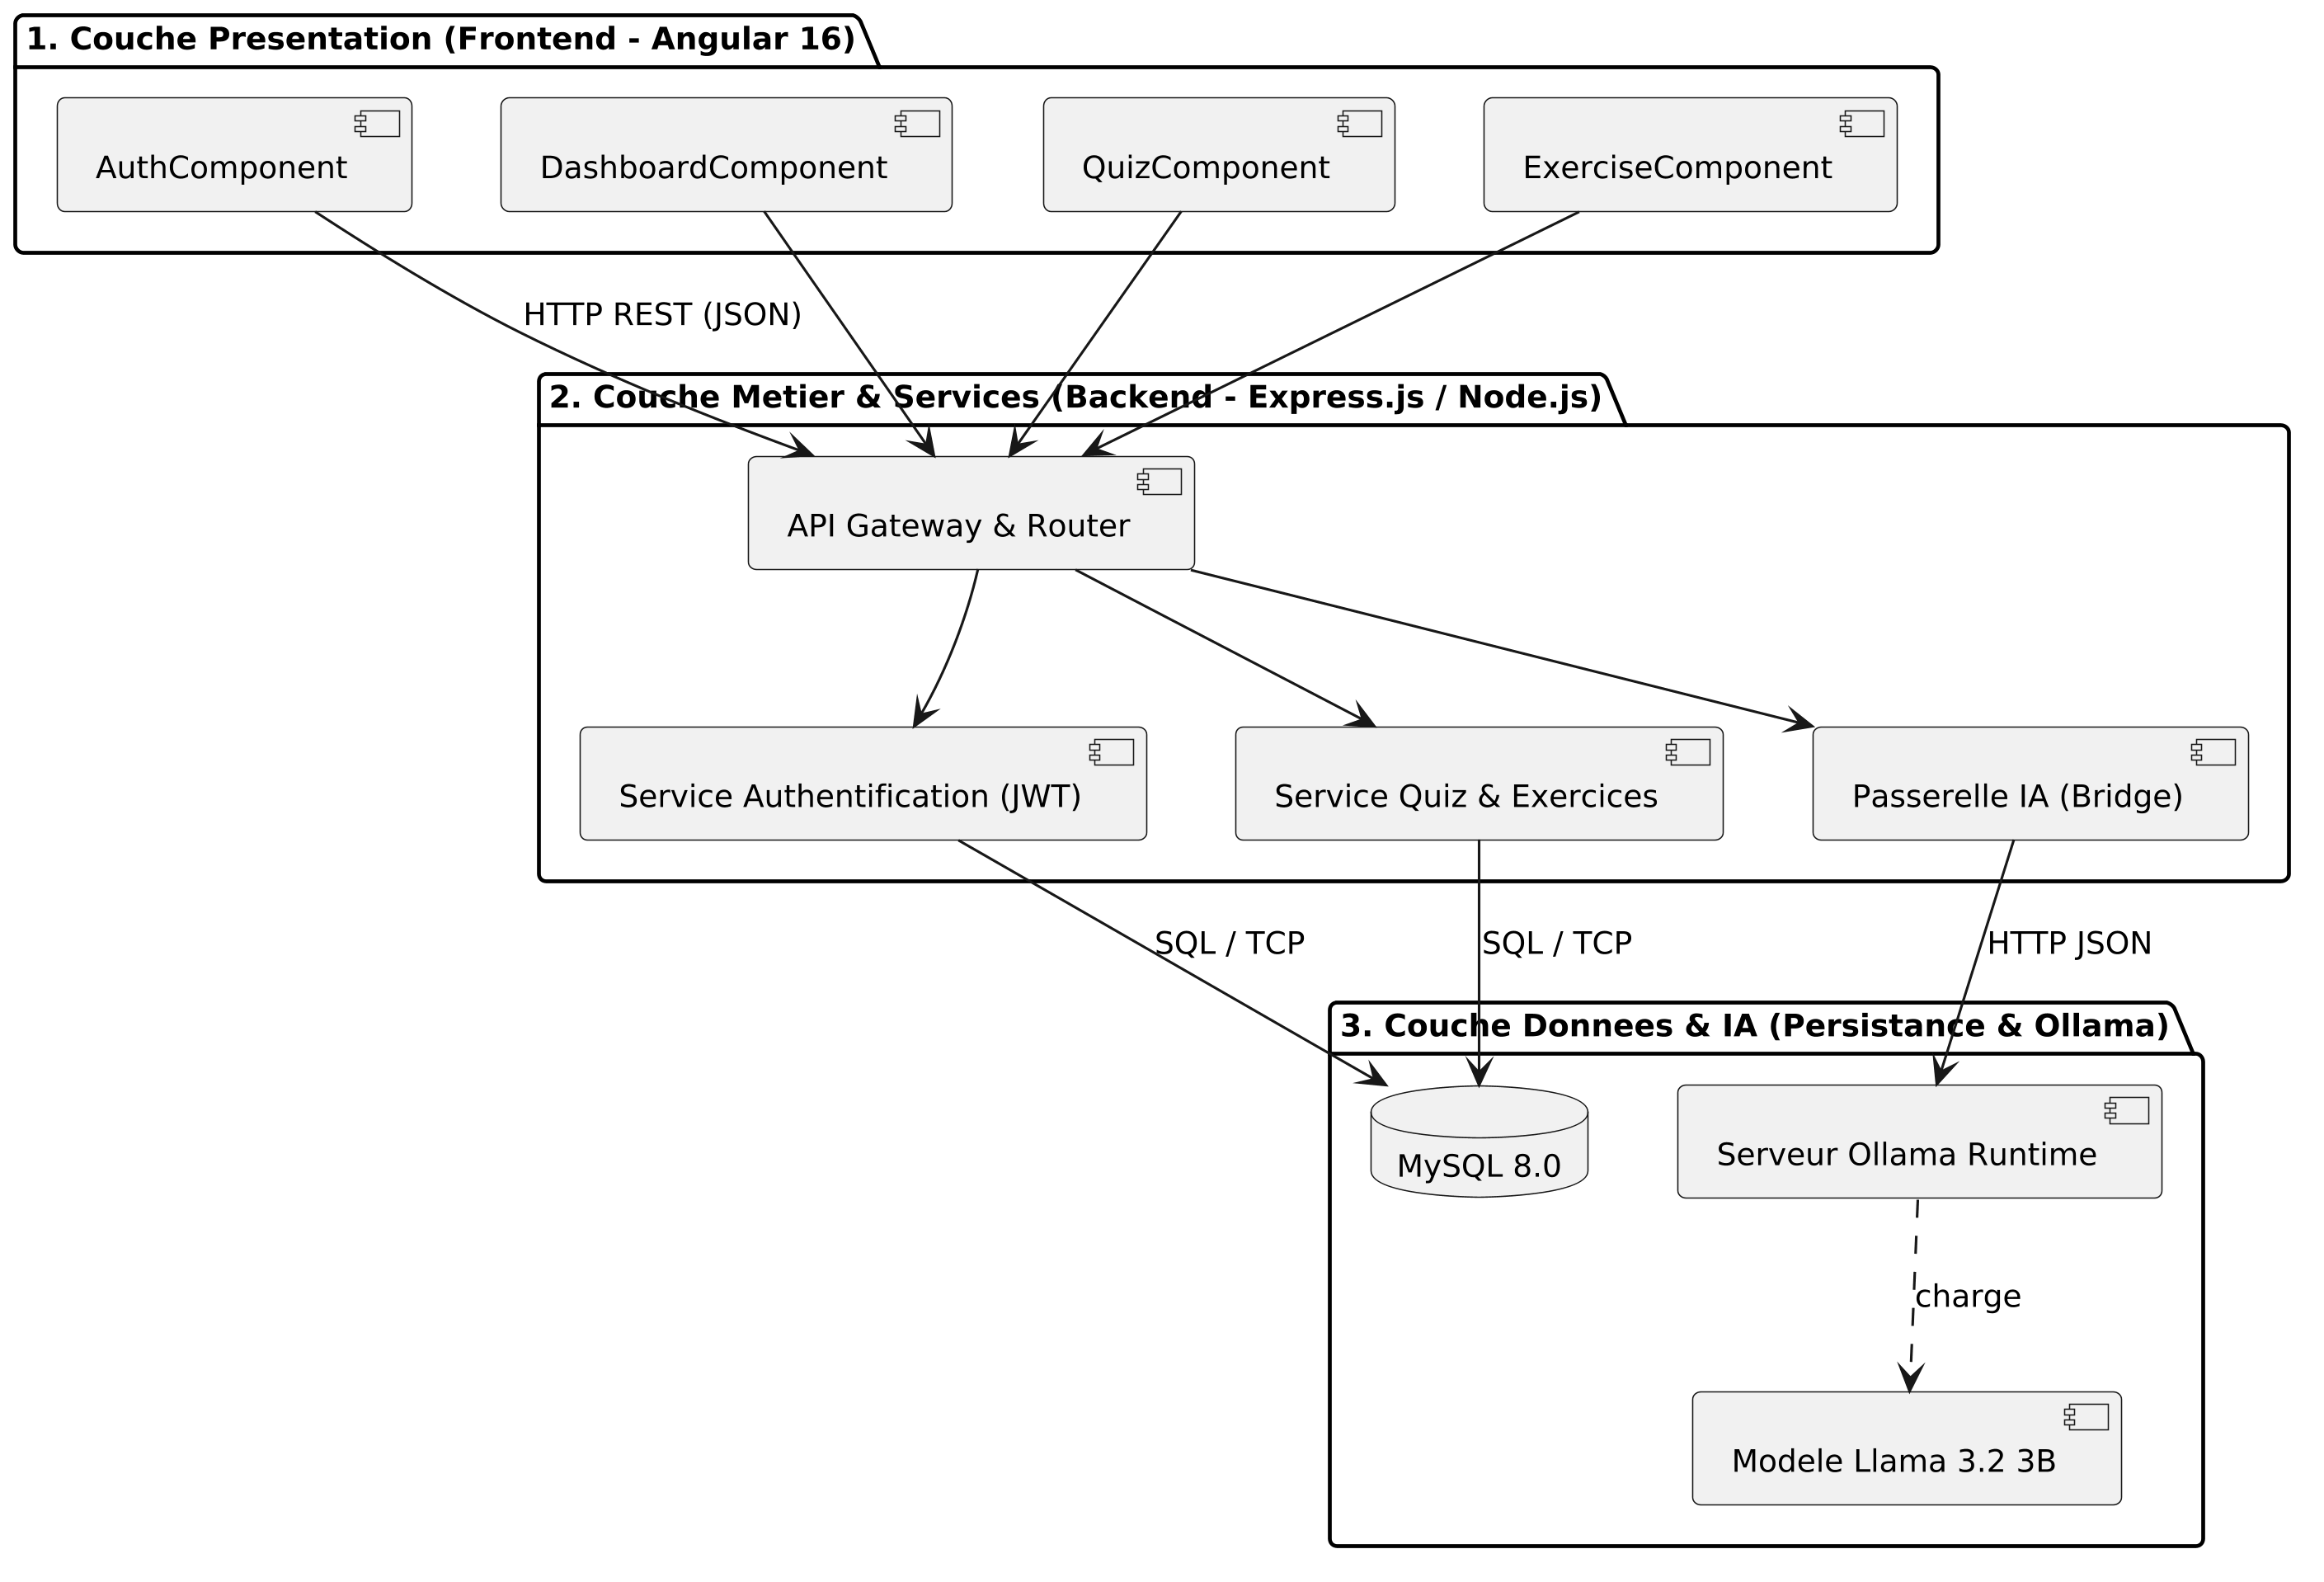
\includegraphics[width=0.95\textwidth,height=11cm,keepaspectratio]{comp_diag.png}%
  }{%
    \fbox{\parbox[c][3.5cm][c]{0.92\textwidth}{\centering
      \textbf{\large [ EMPLACEMENT PHOTO : DIAGRAMME DE COMPOSANTS 3-TIERS ]}\\[8pt]
      \small Déposez votre image dans le dossier et indiquez son nom ci-dessus :\\
      \texttt{\textbackslash includegraphics[width=0.85\textbackslash textwidth]\{comp\_diag.png\}}\\[6pt]
      \footnotesize\itshape Description : Diagramme de composants UML de l'architecture logicielle 3-Tiers.
    }}%
  }
  \caption{Diagramme de composants de l'architecture logicielle 3-Tiers}
  \label{fig:comp_diag}
\end{figure}

\subsubsection{Architecture matériel}
La figure \ref{fig:deploiement} présente le diagramme de déploiement matériel et logiciel, matérialisant les nœuds de calcul et les protocoles de communication réseau.

\begin{figure}[H]
  \centering
  % >>> INSÉREZ VOTRE PHOTO ICI : Remplacez 'deploiement.png' par le nom de votre fichier image <<<
  \IfFileExists{deploiement.png}{%
    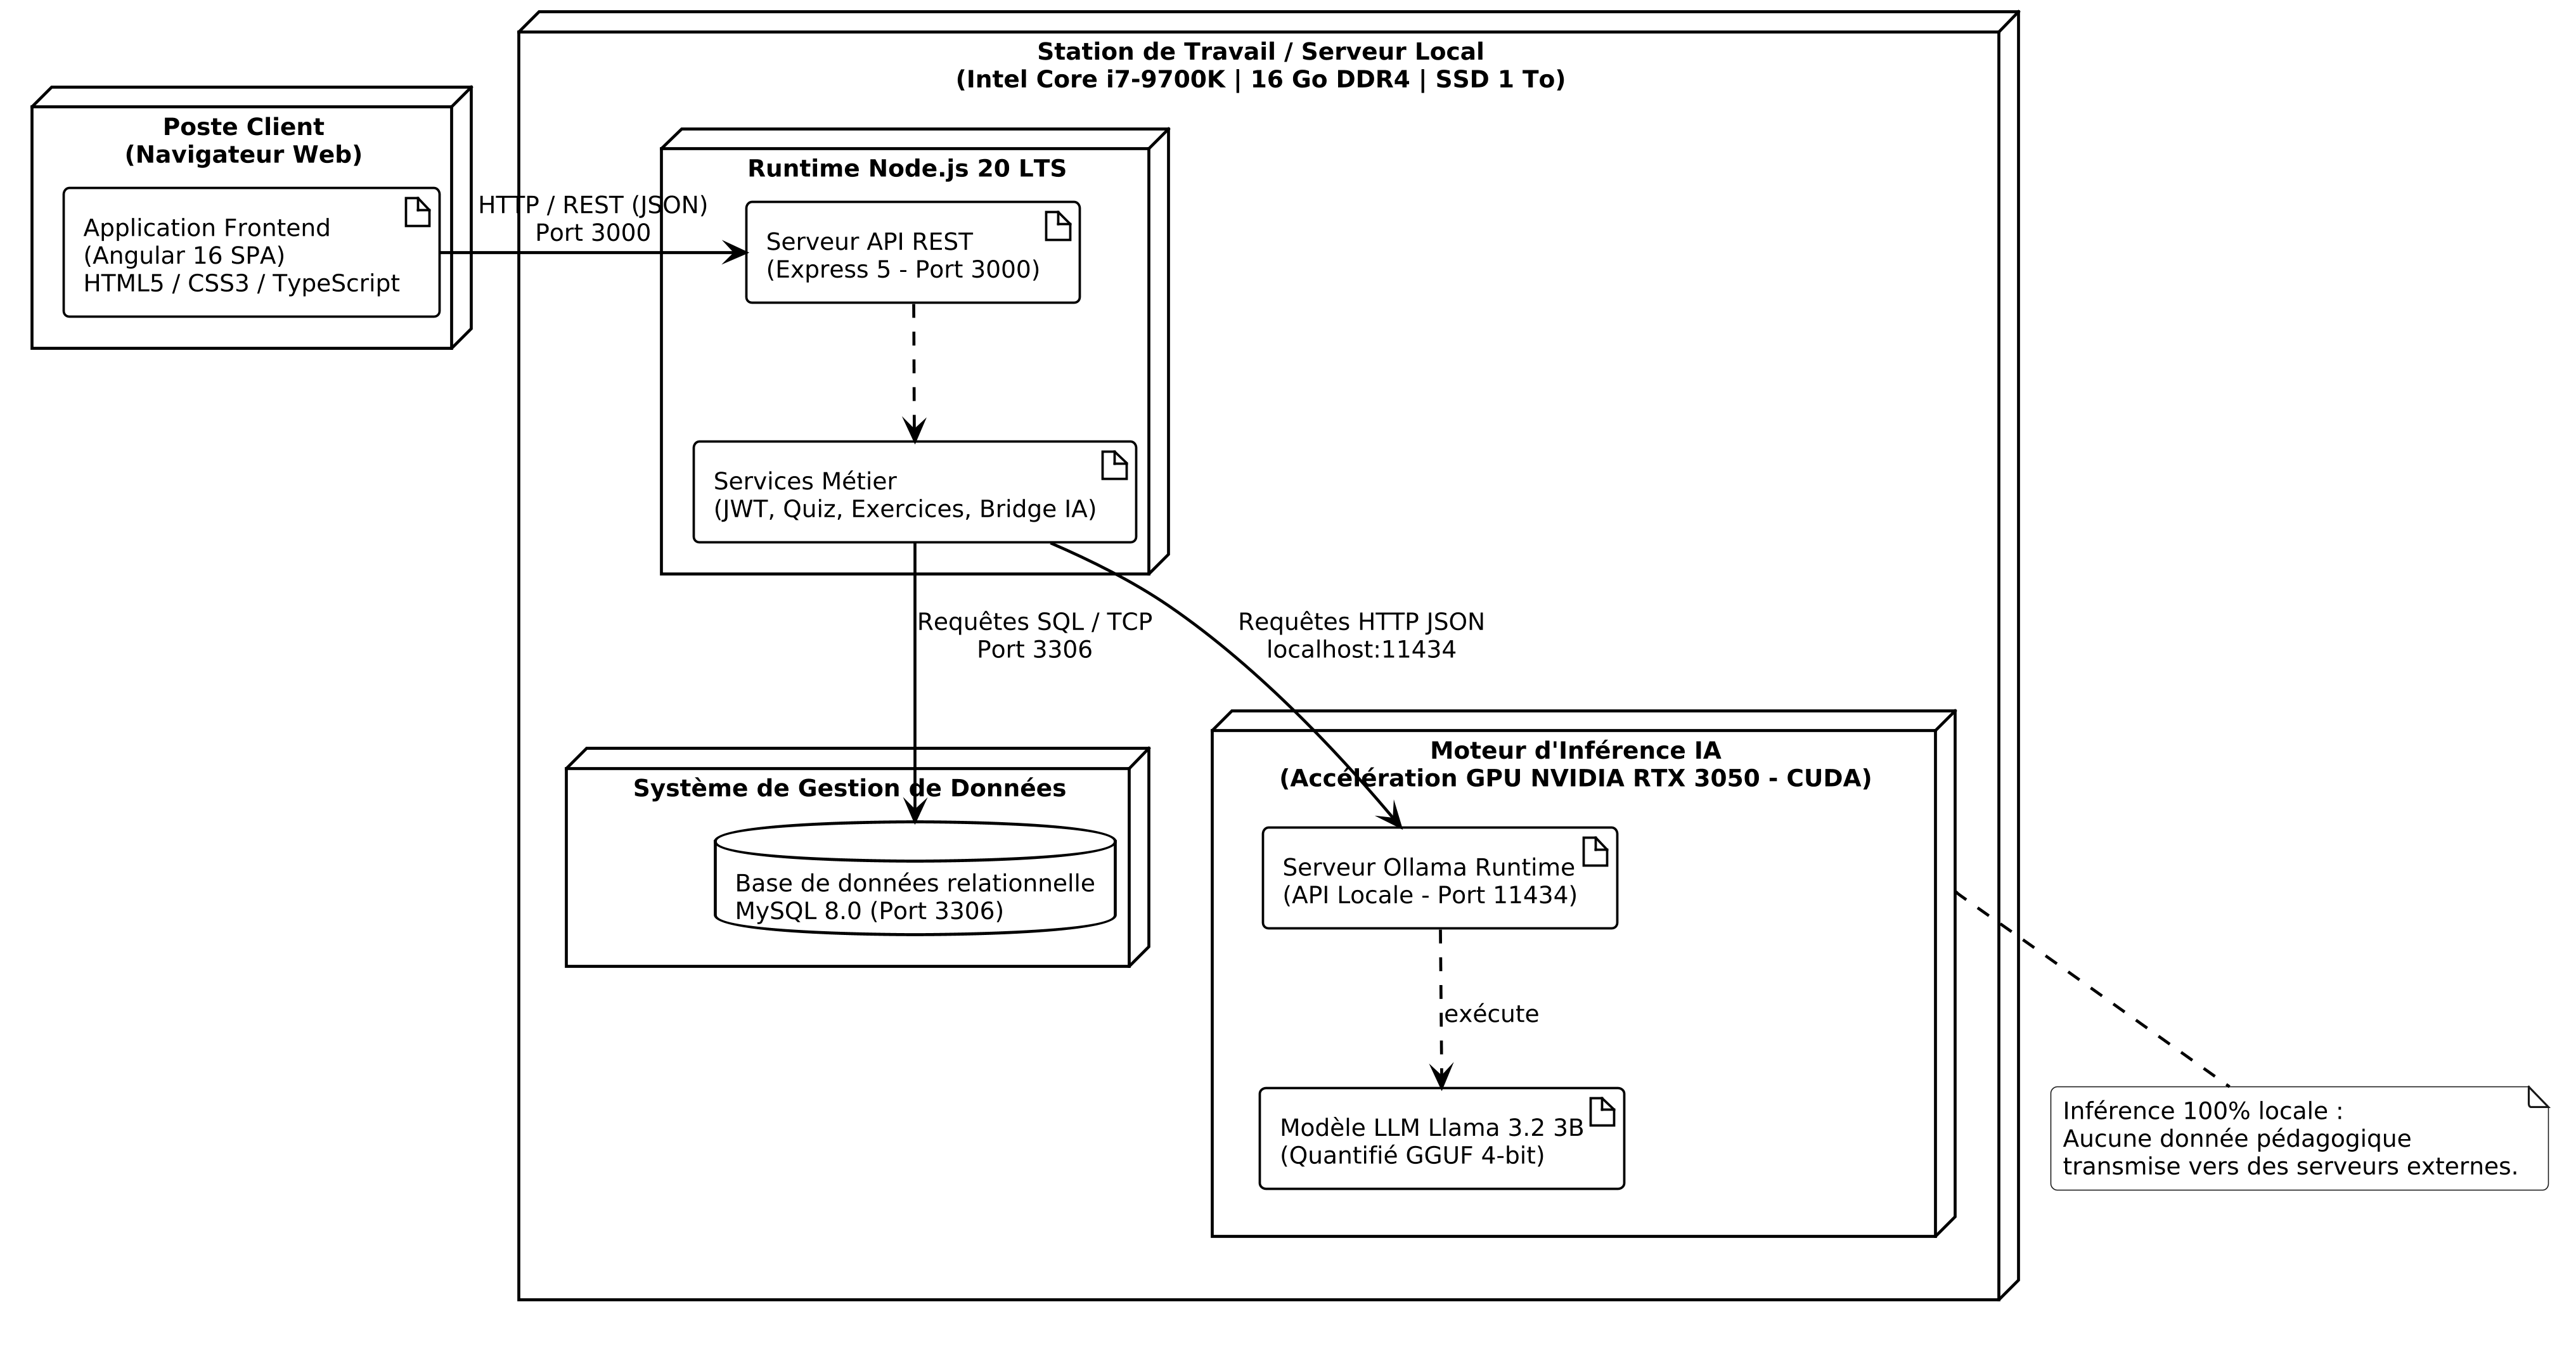
\includegraphics[width=0.95\textwidth,height=12cm,keepaspectratio]{deploiement.png}%
  }{%
    \fbox{\parbox[c][3.5cm][c]{0.92\textwidth}{\centering
      \textbf{\large [ EMPLACEMENT PHOTO : DIAGRAMME DE DÉPLOIEMENT ]}\\[8pt]
      \small Déposez votre image dans le dossier et indiquez son nom ci-dessus :\\
      \texttt{\textbackslash includegraphics[width=0.85\textbackslash textwidth]\{deploiement.png\}}\\[6pt]
      \footnotesize\itshape Description : Diagramme de déploiement matériel et logiciel de la plateforme.
    }}%
  }
  \caption{Diagramme de déploiement matériel et logiciel de la plateforme}
  \label{fig:deploiement}
\end{figure}

\section{Conclusion}
Au terme de ce chapitre, l'architecture logicielle et matérielle de TutorAI a été rigoureusement spécifiée. Les diagrammes de comportement dynamique ont permis de sécuriser le protocole d'évaluation des exercices, tandis que le modèle relationnel garantit une intégrité optimale des données. Nous pouvons désormais aborder la phase de concrétisation et de mise en œuvre dans le chapitre de réalisation.

% ------------------------------------------------------------------------------
% CHAPITRE 4 : RÉALISATION DU SYSTÈME (PAGE 19 DU GUIDE)
% ------------------------------------------------------------------------------
\chaptercoverpage[Réalisation du système]{Réalisation\\ du système}{4}{}

\section{Introduction}
La phase de réalisation concrétise l'ensemble des modélisations et architectures établies lors des étapes antérieures. Ce chapitre expose dans un premier temps l'environnement matériel et logiciel ayant servi de banc de développement. Dans un second temps, nous présentons et commentons les principales interfaces graphiques développées, illustrant le parcours utilisateur complet au sein de TutorAI.

\section{Environnement de développement}

\subsection{Environnement matériel}
Le développement et l'exécution des modèles d'inférence en local ont été menés sur une station de travail dotée des spécifications techniques suivantes :
\begin{itemize}
  \item[—] \textbf{Processeur (CPU) :} Intel Core i7-9700K (8 cœurs / 8 threads) cadencé à 3.6 GHz (Boost jusqu'à 4.9 GHz),
  \item[—] \textbf{Mémoire vive (RAM) :} 16 Go DDR4 assurant une gestion fluide des inférences du modèle de langage en mémoire,
  \item[—] \textbf{Stockage :} Disque SSD de 1 To offrant des temps d'accès rapides aux données et aux modèles Ollama,
  \item[—] \textbf{Accélération graphique (GPU) :} NVIDIA GeForce RTX 3050 avec support CUDA assurant l'accélération matricielle lors des inférences LLM sous Ollama.
\end{itemize}

\subsection{Environnement logiciel}
La suite d'outils et technologies mobilisée comprend :
\begin{itemize}
  \item[—] \textbf{Front-End :} Framework Angular 16, TypeScript 5.1, Angular Material pour les composants visuels réactifs, et TailwindCSS pour l'ergonomie fine des interfaces,
  \item[—] \textbf{Back-End :} Node.js 20 LTS, framework Express 5, pilote MySQL2 avec pool de connexions asynchrones,
  \item[—] \textbf{Intelligence Artificielle :} Moteur Ollama hébergeant le modèle Llama 3.2 (format quantifié GGUF 4-bit) communicant via une API JSON locale,
  \item[—] \textbf{Outils d'ingénierie et tests :} Environnement de développement Visual Studio Code / Antigravity IDE, client Postman pour les tests d'API, système de contrôle de versions Git et serveur web de développement Angular CLI.
\end{itemize}

\section{Principales interfaces graphiques}
Les principales interfaces développées pour la plateforme TutorAI sont présentées et commentées ci-dessous, illustrant le parcours utilisateur complet :

\subsection{Interface du tableau de bord apprenant et progression par matière}
\begin{figure}[H]
  \centering
  % >>> INSÉREZ VOTRE PHOTO / CAPTURE D'ÉCRAN ICI : Remplacez 'ui_dashboard.png' <<<
  \IfFileExists{ui_dashboard.png}{%
    \includegraphics[width=0.95\textwidth,height=10cm,keepaspectratio]{ui_dashboard.png}%
  }{%
    \fbox{\parbox[c][3.5cm][c]{0.92\textwidth}{\centering
      \textbf{\large [ EMPLACEMENT PHOTO : CAPTURE DU TABLEAU DE BORD ]}\\[8pt]
      \small Déposez votre capture dans le dossier et indiquez son nom ci-dessus :\\
      \texttt{\textbackslash includegraphics[width=0.85\textbackslash textwidth]\{ui\_dashboard.png\}}\\[6pt]
      \footnotesize\itshape Description : Capture d'écran du tableau de bord apprenant avec progression par matière et indicateurs de niveau adaptatif.
    }}%
  }
  \caption{Tableau de bord de l'apprenant avec indicateurs de progression adaptative}
  \label{fig:ui_dashboard}
\end{figure}

\noindent
\textit{Description :} Cette interface synthétise la progression pédagogique de l'étudiant à travers des compteurs d'XP, un palier adaptatif calculé dynamiquement et un sélecteur instantané de disciplines. Elle met à disposition un bouton héroïque permettant de solliciter la génération d'un nouvel exercice personnalisé en un clic.

\subsection{Interface de traitement et de saisie d'un exercice pratique}
\begin{figure}[H]
  \centering
  % >>> INSÉREZ VOTRE PHOTO / CAPTURE D'ÉCRAN ICI : Remplacez 'ui_workspace.png' <<<
  \IfFileExists{ui_workspace.png}{%
    \includegraphics[width=0.95\textwidth,height=10cm,keepaspectratio]{ui_workspace.png}%
  }{%
    \fbox{\parbox[c][3.5cm][c]{0.92\textwidth}{\centering
      \textbf{\large [ EMPLACEMENT PHOTO : ESPACE DE TRAVAIL DE L'EXERCICE ]}\\[8pt]
      \small Déposez votre capture dans le dossier et indiquez son nom ci-dessus :\\
      \texttt{\textbackslash includegraphics[width=0.85\textbackslash textwidth]\{ui\_workspace.png\}}\\[6pt]
      \footnotesize\itshape Description : Capture d'écran de l'espace de résolution d'exercice pratique avec auto-sauvegarde.
    }}%
  }
  \caption{Espace de travail et éditeur de réponse à un exercice pratique}
  \label{fig:ui_workspace}
\end{figure}

\noindent
\textit{Description :} L'espace de travail isole distinctement le document d'étude, les questions ordonnées et le champ de rédaction. Il intègre un mécanisme d'auto-sauvegarde en local et des actions d'évaluation immédiates sans nécessiter de rechargement complet de la page.

\subsection{Interface du bilan méthodologique et restitution du corrigé type officiel}
\begin{figure}[H]
  \centering
  % >>> INSÉREZ VOTRE PHOTO / CAPTURE D'ÉCRAN ICI : Remplacez 'ui_correction.png' <<<
  \IfFileExists{ui_correction.png}{%
    \includegraphics[width=0.95\textwidth,height=10cm,keepaspectratio]{ui_correction.png}%
  }{%
    \fbox{\parbox[c][3.5cm][c]{0.92\textwidth}{\centering
      \textbf{\large [ EMPLACEMENT PHOTO : RESTITUTION SANS COMPLAISANCE ET CORRIGÉ ]}\\[8pt]
      \small Déposez votre capture dans le dossier et indiquez son nom ci-dessus :\\
      \texttt{\textbackslash includegraphics[width=0.85\textbackslash textwidth]\{ui\_correction.png\}}\\[6pt]
      \footnotesize\itshape Description : Capture d'écran de la restitution (note 0/100 si non-réponse et affichage du corrigé type officiel).
    }}%
  }
  \caption{Restitution sans complaisance avec affichage du corrigé type officiel}
  \label{fig:ui_correction}
\end{figure}

\noindent
\textit{Description :} Cette interface met en œuvre le principe fondamental d'impartialité pédagogique. Toute réponse évasive est sanctionnée par un score nul (0/100) tout en affichant sans ambiguïté les attendus scientifiques complets afin d'encourager la reprise réflexive de l'exercice.

\subsection{Interface de génération d'exercices sur mesure par le Tuteur IA}
\begin{figure}[H]
  \centering
  % >>> INSÉREZ VOTRE PHOTO / CAPTURE D'ÉCRAN ICI : Remplacez 'ui_gen.png' <<<
  \IfFileExists{ui_gen.png}{%
    \includegraphics[width=0.95\textwidth,height=10cm,keepaspectratio]{ui_gen.png}%
  }{%
    \fbox{\parbox[c][3.5cm][c]{0.92\textwidth}{\centering
      \textbf{\large [ EMPLACEMENT PHOTO : MODALE DE GÉNÉRATION D'EXERCICES ]}\\[8pt]
      \small Déposez votre capture dans le dossier et indiquez son nom ci-dessus :\\
      \texttt{\textbackslash includegraphics[width=0.85\textbackslash textwidth]\{ui\_gen.png\}}\\[6pt]
      \footnotesize\itshape Description : Capture d'écran de la modale de génération paramétrée d'un nouveau cas pratique par le Tuteur IA.
    }}%
  }
  \caption{Modale de génération paramétrée d'un nouveau cas pratique par le Tuteur IA}
  \label{fig:ui_gen}
\end{figure}

\noindent
\textit{Description :} Cette modale permet à l'apprenant d'orienter l'intelligence artificielle locale vers un axe thématique spécifique et de sélectionner un niveau de difficulté adapté, produisant un énoncé et un corrigé inédits en moins de 3 secondes.

\subsection{Interface de génération de quiz par le Tuteur IA}
\begin{figure}[H]
  \centering
  % >>> INSÉREZ VOTRE PHOTO / CAPTURE D'ÉCRAN ICI : Remplacez 'ui_quiz_gen.png' <<<
  \IfFileExists{ui_quiz_gen.png}{%
    \includegraphics[width=0.95\textwidth,height=10cm,keepaspectratio]{ui_quiz_gen.png}%
  }{%
    \fbox{\parbox[c][3.5cm][c]{0.92\textwidth}{\centering
      \textbf{\large [ EMPLACEMENT PHOTO : INTERFACE GÉNÉRATION DE QUIZ ]}\\[8pt]
      \small Déposez votre capture dans le dossier et indiquez son nom ci-dessus :\\
      \texttt{\textbackslash includegraphics[width=0.85\textbackslash textwidth]\{ui\_quiz\_gen.png\}}\\[6pt]
      \footnotesize\itshape Description : Capture d'écran de l'interface de lancement d'un quiz adaptatif avec sélection de la matière, du chapitre et du niveau de difficulté.
    }}%
  }
  \caption{Interface de génération d'un quiz adaptatif par le Tuteur IA}
  \label{fig:ui_quiz_gen}
\end{figure}

\noindent
\textit{Description :} Cette interface constitue le point d'entrée du module d'évaluation par quiz. L'élève sélectionne la matière souhaitée parmi celles de son cursus scolaire (Mathématiques, Français, Arabe, etc.), puis choisit un chapitre ou un thème spécifique. Le système sollicite ensuite le moteur d'intelligence artificielle locale (Ollama -- Llama 3.2) pour générer dynamiquement une série de questions à choix multiples calibrées selon le palier adaptatif de l'apprenant (Débutant, Intermédiaire ou Avancé). Un mécanisme de repli vers une banque certifiée garantit la disponibilité même en cas de charge du serveur LLM.

\subsection{Interface de déroulement d'un quiz -- Questions et réponses}
\begin{figure}[H]
  \centering
  % >>> INSÉREZ VOTRE PHOTO / CAPTURE D'ÉCRAN ICI : Remplacez 'ui_quiz_question.png' <<<
  \IfFileExists{ui_quiz_question.png}{%
    \includegraphics[width=0.95\textwidth,height=10cm,keepaspectratio]{ui_quiz_question.png}%
  }{%
    \fbox{\parbox[c][3.5cm][c]{0.92\textwidth}{\centering
      \textbf{\large [ EMPLACEMENT PHOTO : INTERFACE QUESTION DE QUIZ ]}\\[8pt]
      \small Déposez votre capture dans le dossier et indiquez son nom ci-dessus :\\
      \texttt{\textbackslash includegraphics[width=0.85\textbackslash textwidth]\{ui\_quiz\_question.png\}}\\[6pt]
      \footnotesize\itshape Description : Capture d'écran d'une question de quiz avec les options de réponse, la barre de progression et le minuteur.
    }}%
  }
  \caption{Déroulement interactif d'une question de quiz avec options de réponse}
  \label{fig:ui_quiz_question}
\end{figure}

\noindent
\textit{Description :} L'interface de déroulement du quiz présente chaque question de manière claire et immersive. L'énoncé de la question est affiché en haut de l'écran, accompagné d'un indicateur visuel de progression (numéro de la question courante par rapport au total). Les options de réponse sont disposées sous forme de cartes cliquables, permettant à l'élève de sélectionner sa réponse intuitivement. Un retour visuel immédiat (couleur verte pour la bonne réponse, rouge pour l'erreur) est fourni après chaque validation, accompagné d'une explication pédagogique courte générée par l'IA pour renforcer la compréhension.

\subsection{Interface des résultats finaux du quiz}
\begin{figure}[H]
  \centering
  % >>> INSÉREZ VOTRE PHOTO / CAPTURE D'ÉCRAN ICI : Remplacez 'ui_quiz_results.png' <<<
  \IfFileExists{ui_quiz_results.png}{%
    \includegraphics[width=0.95\textwidth,height=10cm,keepaspectratio]{ui_quiz_results.png}%
  }{%
    \fbox{\parbox[c][3.5cm][c]{0.92\textwidth}{\centering
      \textbf{\large [ EMPLACEMENT PHOTO : RÉSULTATS FINAUX DU QUIZ ]}\\[8pt]
      \small Déposez votre capture dans le dossier et indiquez son nom ci-dessus :\\
      \texttt{\textbackslash includegraphics[width=0.85\textbackslash textwidth]\{ui\_quiz\_results.png\}}\\[6pt]
      \footnotesize\itshape Description : Capture d'écran de l'écran de résultats finaux du quiz avec score, statistiques et message d'encouragement.
    }}%
  }
  \caption{Écran de résultats finaux du quiz avec bilan de performance}
  \label{fig:ui_quiz_results}
\end{figure}

\noindent
\textit{Description :} À l'issue du quiz, cette interface récapitulative affiche le score global obtenu par l'apprenant (nombre de bonnes réponses sur le total), accompagné d'un message d'encouragement personnalisé et bienveillant adapté à la performance. Un récapitulatif question par question permet à l'élève de revisualiser ses réponses et les corrections associées. Le système attribue automatiquement les points d'expérience (XP) gagnés et met à jour le palier adaptatif en conséquence, valorisant chaque effort fourni par l'élève.

\subsection{Interface de suivi de la progression de l'apprenant}
\begin{figure}[H]
  \centering
  % >>> INSÉREZ VOTRE PHOTO / CAPTURE D'ÉCRAN ICI : Remplacez 'ui_progression.png' <<<
  \IfFileExists{ui_progression.png}{%
    \includegraphics[width=0.95\textwidth,height=10cm,keepaspectratio]{ui_progression.png}%
  }{%
    \fbox{\parbox[c][3.5cm][c]{0.92\textwidth}{\centering
      \textbf{\large [ EMPLACEMENT PHOTO : INTERFACE DE PROGRESSION ]}\\[8pt]
      \small Déposez votre capture dans le dossier et indiquez son nom ci-dessus :\\
      \texttt{\textbackslash includegraphics[width=0.85\textbackslash textwidth]\{ui\_progression.png\}}\\[6pt]
      \footnotesize\itshape Description : Capture d'écran du tableau de suivi de progression avec statistiques par matière, historique des quiz et exercices complétés.
    }}%
  }
  \caption{Tableau de suivi de la progression pédagogique par matière}
  \label{fig:ui_progression}
\end{figure}

\noindent
\textit{Description :} Le module de progression offre une vue synthétique et détaillée de l'évolution pédagogique de l'élève. Pour chaque matière, l'interface affiche le nombre de quiz et d'exercices complétés, la moyenne générale obtenue, le palier adaptatif courant (Débutant, Intermédiaire ou Avancé) et le total de points d'expérience accumulés. Des indicateurs visuels sous forme de barres de progression et de badges colorés permettent à l'apprenant de visualiser concrètement ses avancées. Ce suivi longitudinal encourage la persévérance et permet aux parents de consulter les progrès de leur enfant en un coup d'œil.

\section{Conclusion}
La concrétisation logicielle de TutorAI a permis de valider l'adéquation entre l'architecture conceptuelle définie et les exigences fonctionnelles réelles. Grâce à l'association d'Angular 16 et du moteur d'inférence LLM local, l'application concilie réactivité d'affichage, rigueur pédagogique et souveraineté des données académiques.

% ------------------------------------------------------------------------------
% CONCLUSION GÉNÉRALE (PAGE 21 DU GUIDE - EN UNE PAGE SOUS FORME D'UN PARAGRAPHE UNIQUE SANS TIRETS)
% ------------------------------------------------------------------------------
\chapter*{Conclusion générale}
\addcontentsline{toc}{chapter}{Conclusion générale}
\markboth{Conclusion générale}{Conclusion générale}

Le stage de perfectionnement effectué du 1\textsuperscript{er} juillet au 1\textsuperscript{er} août 2026 au sein de la société UQASE NEXT SARL à Casablanca a constitué une expérience professionnelle et humaine particulièrement enrichissante, nous permettant de mobiliser l'ensemble des compétences méthodologiques, algorithmiques et architecturales acquises tout au long de notre cursus d'ingénierie informatique et réseaux à l'École Marocaine des Sciences de l'Ingénieur (EMSI). En réponse aux défis majeurs de l'échec scolaire précoce et du manque de soutien personnalisé pour les enfants et adolescents (âgés de 6 à 15 ans, cycles primaire et collège) en difficulté d'apprentissage, nous avons mené à bien la conception et la réalisation de la plateforme web innovante TutorAI. Ce système associe harmonieusement un écosystème front-end réactif et ludifié sous Angular 16, une API REST robuste sous Node.js/Express et un serveur d'inférence d'intelligence artificielle locale exploitant le modèle de langage Llama 3.2 sous Ollama, garantissant la stricte confidentialité des données des élèves mineurs. Les objectifs fixés au cahier des charges ont été pleinement atteints, notamment la mise en place d'un parcours diagnostique bienveillant, d'un moteur de quiz et d'exercices à paliers adaptatifs, d'un agent tuteur doué d'empathie pédagogique et d'un mécanisme de remédiation décomposant pas-à-pas les solutions pour débloquer l'élève sans le décourager. Grâce à la conduite du projet sous la méthodologie Agile Scrum et sous la supervision bienveillante de notre encadrante professionnelle, Madame Aïcha FADLI, Responsable Digitale, nous avons pu rythmer nos livraisons logicielles avec rigueur tout au long de ce mois intensif de stage estival. Avec un regard critique constructif sur nos réalisations, nous relevons des pistes d'évolution prometteuses, notamment l'intégration d'un module d'interaction vocale basé sur Whisper particulièrement adapté aux plus jeunes enfants ayant des difficultés en lecture, l'enrichissement documentaire par RAG adossé aux manuels scolaires officiels, et le renforcement des tableaux de bord parentaux pour un suivi longitudinal des progrès. En définitive, ce travail d'ingénierie logicielle confirme notre volonté de mettre l'intelligence artificielle au service d'une cause éducative et humaine essentielle : redonner confiance et plaisir d'apprendre à chaque élève en difficulté.

% ------------------------------------------------------------------------------
% BIBLIOGRAPHIE ET NÉTOGRAPHIE (PAGE 22 DU GUIDE)
% ------------------------------------------------------------------------------
\chapter*{Bibliographie et Nétographie}
\addcontentsline{toc}{chapter}{Bibliographie et Nétographie}
\markboth{Bibliographie et Nétographie}{Bibliographie et Nétographie}

\section*{Bibliographie}
\begin{enumerate}
  \item[1.] \textsc{Roques}, Pascal. « UML 2 par la pratique : Études de cas et exercices corrigés », Paris, Éditions Eyrolles, 2006, 380 pages.
  \item[2.] \textsc{Reeves}, Hubert. « Bases de données relationnelles », Paris, Éditions du Seuil, 1988, 250 pages.
  \item[3.] \textsc{Audibert}, Laurent. « UML 2 : De l'apprentissage à la pratique », Paris, Éditions Ellipses, 2009, 288 pages.
  \item[4.] \textsc{Gamma}, Erich, \textsc{Helm}, Richard, \textsc{Johnson}, Ralph, et \textsc{Vlissides}, John. « Design Patterns : Catalogue de modèles de conception réutilisables », Paris, Vuibert, 1999, 496 pages.
\end{enumerate}

\section*{Nétographie}
\begin{enumerate}
  \item[1.] \url{https://angular.io/docs} : Documentation technique officielle du framework Angular et des composants standalone.
  \item[2.] \url{https://nodejs.org/en/docs/} : Références officielles de l'environnement d'exécution Node.js et architecture asynchrone.
  \item[3.] \url{https://ollama.ai/} : Documentation du moteur d'inférence local de modèles de langage et intégration d'API JSON.
  \item[4.] \url{https://expressjs.com/} : Guide d'architecture et de routage pour le framework web Express.
  \item[5.] \url{https://www.uml-diagrams.org/} : Ressources et spécifications normatives des diagrammes du standard UML 2.5.
\end{enumerate}

% ------------------------------------------------------------------------------
% ANNEXES (PAGES 23-27 DU GUIDE)
% ------------------------------------------------------------------------------
\appendix

\chapter*{ANNEXES}
\addcontentsline{toc}{chapter}{ANNEXES}
\markboth{ANNEXES}{ANNEXES}

\noindent
\textbf{ANNEXE A : Module d'interception algorithmique des non-réponses}\newline
\textbf{ANNEXE B : Configuration et déploiement conteneurisé (Docker)}

\newpage
\chapter*{ANNEXE A : Module d'interception algorithmique des non-réponses}
\addcontentsline{toc}{chapter}{ANNEXE A : Module d'interception algorithmique des non-réponses}
\markboth{ANNEXE A : Module d'interception algorithmique des non-réponses}{ANNEXE A : Module d'interception algorithmique des non-réponses}

Cette annexe détaille l'implémentation algorithmique de la fonction de filtrage et d'interception des réponses évasives développée au sein du backend de la plateforme TutorAI.

\section*{Module d'interception stricte des non-réponses (JavaScript)}
L'extrait suivant, issu du service \texttt{ai-quiz-exercise.service.js}, implémente la détection algorithmique des expressions d'incompréhension ou de refus afin d'éviter toute complaisance évaluative :

\begin{lstlisting}[language=Java, caption={Fonction de d\'etection des non-r\'eponses et aveux d'incompr\'ehension}]
function isNonAnswer(text) {
  if (!text) return true;
  const raw = String(text).trim();
  if (raw.length === 0) return true;

  // Normalisation des accents et ponctuation
  const clean = raw
    .toLowerCase()
    .normalize('NFD')
    .replace(/[\u0300-\u036f]/g, '')
    .replace(/[.,\/#!$%\^&\*;:{}=\-_`~()?'"\u00AB\u00BB\\]/g, ' ')
    .replace(/\s+/g, ' ')
    .trim();

  if (!clean || clean.length === 0) return true;

  const nonAnswerExact = new Set([
    'jsp', 'jsais pas', 'j sais pas', 'je sais pas', 'je ne sais pas', 'sais pas',
    'chepa', 'che pas', 'chpa', 'idk', 'i dont know', 'dont know',
    'rien', 'rien du tout', 'aucun', 'aucune', 'aucune idee', 'pas compris',
    'aide moi', 'help', 'sos', 'bloque', 'bof', 'non', 'null', 'vide', 'test'
  ]);

  if (nonAnswerExact.has(clean)) return true;
  if (/^(.)\1*$/.test(clean) && clean.length < 15) return true;
  if (/^(jsp|idk|rien|aide)\b/i.test(clean) && clean.length <= 15) return true;
  if (/^je\s*(ne\s*)?sais\s*pas/i.test(clean) && clean.length <= 25) return true;

  return false;
}
\end{lstlisting}

\newpage
\chapter*{ANNEXE B : Configuration et déploiement Docker}
\addcontentsline{toc}{chapter}{ANNEXE B : Configuration et déploiement Docker}
\markboth{ANNEXE B : Configuration et déploiement Docker}{ANNEXE B : Configuration et déploiement Docker}

Le fichier \texttt{docker-compose.yml} assure l'instanciation conjointe du serveur de base de données MySQL 8 et du moteur d'inférence d'IA Ollama :

\begin{lstlisting}[language=XML, caption={Fichier docker-compose.yml pour l'environnement local}]
version: '3.8'

services:
  database:
    image: mysql:8.0
    container_name: tutorai-mysql
    restart: always
    environment:
      MYSQL_ROOT_PASSWORD: root_secure_password
      MYSQL_DATABASE: tutorai
    ports:
      - "3306:3306"
    volumes:
      - mysql_data:/var/lib/mysql

  ollama-engine:
    image: ollama/ollama:latest
    container_name: tutorai-ollama
    restart: unless-stopped
    ports:
      - "11434:11434"
    volumes:
      - ollama_models:/root/.ollama

volumes:
  mysql_data:
  ollama_models:
\end{lstlisting}

% ==============================================================================
% FIN DU DOCUMENT
% ==============================================================================
\end{document}
